%============================================================================
% PREAMBLE COMPLETO — TMS/DMS/CMS Usage Guide for Falcon BMS 4.38.1
% Gerado: 11 February 2026
% Status: Improvements as per GitHub Issues #34 and #33
%============================================================================

\documentclass[11pt, a4paper, twoside]{report}

% --------------------------------------------------------------------------
% BASIC ENCODING AND LANGUAGE
% --------------------------------------------------------------------------

\usepackage[utf8]{inputenc}
\usepackage[T1]{fontenc}
\usepackage[english]{babel}

% --------------------------------------------------------------------------
% FONTS AND MICROTYPOGRAPHY
% --------------------------------------------------------------------------

\usepackage{lmodern}
\usepackage{microtype}

% --------------------------------------------------------------------------
% PAGE GEOMETRY AND LAYOUT
% --------------------------------------------------------------------------

\usepackage{geometry}
\geometry{a4paper, left=2.0cm, right=2.0cm, top=2.5cm, bottom=2.5cm}
\usepackage{setspace}
\onehalfspacing

% --------------------------------------------------------------------------
% COLORS AND LINKS AND PDF SETTINGS
% --------------------------------------------------------------------------

\usepackage[table]{xcolor}
\definecolor{linkblue}{HTML}{004488}
\definecolor{linkred}{HTML}{882222}
\definecolor{headerblue}{HTML}{003366}
\definecolor{rowgray}{HTML}{F5F5F5}
\definecolor{subheadgray}{HTML}{E0E0E0}
\usepackage{soul}
\usepackage[pdfencoding=auto, psdextra, colorlinks=true, linkcolor=linkblue, citecolor=linkred, urlcolor=linkblue, breaklinks=true]{hyperref}
\hypersetup{
	pdftitle={TMS, DMS and CMS Usage Guide for Falcon BMS},
	pdfauthor={Carlos "Metal" Nader},
	pdfsubject={Flight Simulation - Falcon BMS HOTAS Reference},
	pdfkeywords={Falcon BMS, F-16, HOTAS, TMS, DMS, CMS, Flight Simulation},
	pdfcreator={pdfLaTeX (MiKTeX)},
	pdfproducer={MiKTeX},
	pdflang={en-US},
}
\usepackage{bookmark}

% --------------------------------------------------------------------------
% CAPTION SETUP BY TYPE
% --------------------------------------------------------------------------

\usepackage{caption}

% GLOBAL PATTERN
\captionsetup{font=small, labelfont=bf, justification=centering, singlelinecheck=true}
% FIGURES
\captionsetup[figure]{font=footnotesize, labelfont=bf, justification=centering, singlelinecheck=true}
% % TABLE/LONGTABLE/hotastable:
\captionsetup[table]{font=small, labelfont=bf, justification=centering, singlelinecheck=true}

% --------------------------------------------------------------------------
% HEADERS AND FOOTERS (IMPROVED for report + twoside)
% --------------------------------------------------------------------------

\usepackage{fancyhdr}
\setlength{\headheight}{25pt}                    
\pagestyle{fancy}
\fancyhf{}                                        
\fancyhead[LO,RE]{\small\textit{\leftmark}}     
\fancyhead[RO,LE]{\small\thepage}               
\fancyfoot{}                                      
\renewcommand{\headrulewidth}{0.4pt}
\renewcommand{\footrulewidth}{0pt}

% --------------------------------------------------------------------------
% CHAPTER FORMATTING AND SPACING (via titlesec)
% --------------------------------------------------------------------------

\usepackage{titlesec}

% --------------------------------------------------------------------------
% CHAPTER - Nível 0 (Destaque Máximo)
% --------------------------------------------------------------------------
% Shape: display → standalone em nova linha
% Font: \Large\bfseries --- label e título ambos em bold para destaque máximo
% Numeração: SIM
% Espaçamento: 15pt antes, 28pt depois
% --------------------------------------------------------------------------

\titleformat{\chapter}[display]
{\normalfont\Large\bfseries}           % Formato: LARGE + bold (label)
{\chaptertitlename~\thechapter}        % Rótulo: "Chapter 1" (bold também)
{20pt}                                 % Espaço vertical antes do corpo
{\Large\bfseries}                      % Corpo do título: LARGE + bold

\titlespacing{\chapter}
{0pt}       % Margem esquerda (sem indent)
{15pt}      % Espaço ANTES do título do capítulo
{28pt}      % Espaço DEPOIS do título do capítulo (AUMENTADO)
[0pt]       % Margem direita

% --------------------------------------------------------------------------
% SECTION - Nível 1
% --------------------------------------------------------------------------
% Shape: hang → label à esquerda, corpo indentado (compacto)
% Font: \large\bfseries (mesmo destaque que chapter para coerência)
% Numeração: SIM
% Espaçamento: 15pt antes, 8pt depois (REDUZIDO de 15pt/10pt anteriores)
% --------------------------------------------------------------------------

\titleformat{\section}[hang]
{\normalfont\large\bfseries}           % Formato: large + bold
{\thesection}                          % Rótulo: "1", "2", etc
{1em}                                  % Espaço entre rótulo e corpo
{}                                     % Corpo do título (herda do format)

\titlespacing{\section}
{0pt}       % Margem esquerda (sem indent)
{15pt}      % Espaço ANTES do título da seção (REDUZIDO)
{8pt}       % Espaço DEPOIS do título da seção (REDUZIDO)
[0pt]       % Margem direita

% --------------------------------------------------------------------------
% SUBSECTION - Nível 2
% --------------------------------------------------------------------------
% Shape: hang → label esquerda, corpo indentado
% Font: \normalsize\bfseries (redução visual, ainda robusto)
% Numeração: SIM
% Espaçamento: 12pt antes, 6pt depois (compacto)
% --------------------------------------------------------------------------

\titleformat{\subsection}[hang]
{\normalfont\normalsize\bfseries}      % Formato: tamanho normal + bold
{\thesubsection}                       % Rótulo: "1.1", "1.2", etc
{1em}                                  % Espaço entre rótulo e corpo
{}                                     % Corpo do título

\titlespacing{\subsection}
{0pt}       % Margem esquerda (sem indent)
{12pt}      % Espaço ANTES do título da subseção
{6pt}       % Espaço DEPOIS do título da subseção
[0pt]       % Margem direita

% --------------------------------------------------------------------------
% SUBSUBSECTION - Nível 3
% --------------------------------------------------------------------------
% Shape: hang → label esquerda, máximo recuo (bem compacto)
% Font: \normalsize\bfseries (mesmo tamanho que subsection, padrão)
% Numeração: SIM (configurable com secnumdepth)
% Espaçamento: 10pt antes, 4pt depois (bem comprimido)
% --------------------------------------------------------------------------

\titleformat{\subsubsection}[hang]
{\normalfont\normalsize\bfseries}      % Formato: tamanho normal + bold
{\thesubsubsection}                    % Rótulo: "1.1.1", "1.1.2", etc
{1em}                                  % Espaço entre rótulo e corpo
{}                                     % Corpo do título

\titlespacing{\subsubsection}
{0pt}       % Margem esquerda (sem indent)
{10pt}       % Espaço ANTES do título
{4pt}       % Espaço DEPOIS do título (bem comprimido)
[0pt]       % Margem direita

% --------------------------------------------------------------------------
% PARAGRAPH - Nível 4 (CRÍTICO: Ilusão Óptica Resolvida)
% --------------------------------------------------------------------------
% Shape: runin → inline, integrado ao texto (seu requisito)
% Font: \small\bfseries (SOLUÇÃO PARA ILUSÃO ÓPTICA DO NEGRITO)%       
% Numeração: NÃO (padrão para \paragraph)
% Espaçamento: runin (sem espaço vertical antes, integrado ao texto)
% --------------------------------------------------------------------------

\titleformat{\paragraph}[runin]
{\normalfont\small\bfseries}           % Formato: SMALL + bold (compensa ilusão)
{}                                     % Rótulo: vazio (sem numeração)
{0em}                                  % Espaço entre rótulo e corpo (zero, runin)
{}                                     % Corpo do título

\titlespacing{\paragraph}
{0pt}       % Margem esquerda (sem indent)
{8pt}       % Espaço ANTES do título do parágrafo (ADICIONADO - cria separação)
{1em}       % Espaço DEPOIS do título (ADICIONADO - espaço após ":")
[0pt]       % Margem direita

% --------------------------------------------------------------------------
% SUBPARAGRAPH - Nível 5 (Preparação Futura)
% --------------------------------------------------------------------------
% Shape: runin → inline, integrado ao texto
% Font: \small (MENOS destaque que \paragraph, sem bold)
% Numeração: NÃO (padrão para \subparagraph)
% Espaçamento: runin (integrado)
% Uso: Se usado, aparecerá com destaque menor que \paragraph
% --------------------------------------------------------------------------

\titleformat{\subparagraph}[runin]
{\normalfont\small}                    % Formato: small, SEM bold (menos destaque)
{}                                     % Rótulo: vazio (sem numeração)
{0em}                                  % Espaço entre rótulo e corpo (zero, runin)
{}                                     % Corpo do título

\titlespacing{\subparagraph}
{0pt}       % Margem esquerda (sem indent)
{8pt}       % Espaço ANTES do título (ADICIONADO)
{1em}       % Espaço DEPOIS do título (ADICIONADO)
[0pt]       % Margem direita

% --------------------------------------------------------------------------
% TABLES AND MACROS
% --------------------------------------------------------------------------

\usepackage{booktabs}
\usepackage{array}
\usepackage{longtable}
\usepackage{tabularx}

% Custom Columns
\newcolumntype{L}[1]{>{\raggedright\arraybackslash}p{#1}}
\newcolumntype{C}[1]{>{\centering\arraybackslash}p{#1}}
\newcolumntype{R}[1]{>{\raggedleft\arraybackslash}p{#1}}

% Macro for Visual Reference Links
\newcommand{\imglink}[1]{\hspace{2pt}\hyperref[#1]{\scriptsize\textbf{[Fig]}}}

% --------------------------------------------------------------------------
% HOTAS LOT FILE HANDLE 
% --------------------------------------------------------------------------
\makeatletter
\newcommand{\listofhotastables}{%
	\section*{List of HOTAS Tables}%
	\addcontentsline{toc}{section}{List of HOTAS Tables}%
	\@starttoc{hotas}%
}
\makeatother

% --------------------------------------------------------------------------
% HOTAS table environment
% Version: 2.1 (2026-02-10)
% --------------------------------------------------------------------------

\newenvironment{hotastable}[1]{%
	\footnotesize
	\setlength{\tabcolsep}{3pt}
	\renewcommand{\arraystretch}{1.35}
	\begin{longtable}{L{1.00cm} L{0.90cm} L{0.90cm} L{3.30cm} L{6.40cm} L{1.40cm} L{1.60cm}}
		\caption{#1}\label{table.\thetable}\\
		\noalign{\addtocontents{hotas}{\protect\contentsline{table}{\protect\numberline{\thetable}#1}{\thepage}{table.\thetable}}}%
		\rowcolor{headerblue}
		\multicolumn{1}{>{\centering\arraybackslash}p{1.00cm}}{\textbf{\color{white}Mode}} &
		\multicolumn{1}{>{\centering\arraybackslash}p{0.90cm}}{\textbf{\color{white}Dir.}} &
		\multicolumn{1}{>{\centering\arraybackslash}p{0.90cm}}{\textbf{\color{white}Act.}} &
		\multicolumn{1}{>{\centering\arraybackslash}p{3.30cm}}{\textbf{\color{white}Function}} &
		\multicolumn{1}{>{\centering\arraybackslash}p{6.40cm}}{\textbf{\color{white}Effect / Nuance}} &
		\multicolumn{1}{>{\centering\arraybackslash}p{1.40cm}}{\textbf{\color{white}Dash34}} &
		\multicolumn{1}{>{\centering\arraybackslash}p{1.60cm}}{\textbf{\color{white}Train.}} \\
		\endfirsthead
		\rowcolor{headerblue}
		\multicolumn{1}{>{\centering\arraybackslash}p{1.00cm}}{\textbf{\color{white}Mode}} &
		\multicolumn{1}{>{\centering\arraybackslash}p{0.90cm}}{\textbf{\color{white}Dir.}} &
		\multicolumn{1}{>{\centering\arraybackslash}p{0.90cm}}{\textbf{\color{white}Act.}} &
		\multicolumn{1}{>{\centering\arraybackslash}p{3.30cm}}{\textbf{\color{white}Function}} &
		\multicolumn{1}{>{\centering\arraybackslash}p{6.40cm}}{\textbf{\color{white}Effect / Nuance}} &
		\multicolumn{1}{>{\centering\arraybackslash}p{1.40cm}}{\textbf{\color{white}Dash34}} &
		\multicolumn{1}{>{\centering\arraybackslash}p{1.60cm}}{\textbf{\color{white}Train.}} \\
		\endhead
		\multicolumn{7}{r}{\small\emph{Continued on next page}}\\
		\endfoot
		\endlastfoot
	}{%
	\end{longtable}
}

% --------------------------------------------------------------------------
% SIMPLE REFERENCE MACROS FOR BMS DOCS
% --------------------------------------------------------------------------

\newcommand{\dashref}[1]{Dash-34~\S~#1}
\newcommand{\dashone}[1]{Dash-1~\S~#1}
\newcommand{\trnref}[1]{TRN~#1}
\newcommand{\trnman}{BMS Training Manual 4.38.1}
\newcommand{\bmsver}{Falcon BMS~4.38.1}
\newcommand{\dashrefs}[1]{\textit{TO 1F-16CMAM-34-1-1}, Dash-34, sections \texttt{#1}}

% --------------------------------------------------------------------------
% CROSS-REFERENCE MACROS (INTERNAL GUIDE)
% --------------------------------------------------------------------------

\newcommand{\secref}[1]{\hyperref[#1]{Section~\ref*{#1}}}
\newcommand{\chapref}[1]{\hyperref[#1]{Chapter~\ref*{#1}}}
\newcommand{\tabref}[1]{\hyperref[#1]{Table~\ref*{#1}}}
\newcommand{\figref}[1]{\hyperref[#1]{Figure~\ref*{#1}}}

% --------------------------------------------------------------------------
% VERSION CONTROL MACROS
% --------------------------------------------------------------------------

\newcommand{\docversion}{0.4.1.1}
\newcommand{\docbuild}{20260218}
\newcommand{\docstartdate}{05 January 2026}
\newcommand{\docenddate}{18 February 2026}
\newcommand{\chapterscompletedof}{4/7}
\newcommand{\tablesfilledpct}{Chapter 5 and Chapter 4}
\newcommand{\fulldocversion}{\docversion+\docbuild}

% --------------------------------------------------------------------------
% GRAPHICS
% --------------------------------------------------------------------------

\usepackage{graphicx}
\graphicspath{{fig/}}
\usepackage{float}
\usepackage{enumitem}

% --------------------------------------------------------------------------
% TITLE
% --------------------------------------------------------------------------

\title{TMS, DMS and CMS Usage Guide for \bmsver}
\author{Carlos ``Metal'' Nader}
\date{Version \fulldocversion{} | Progress: Chapters \chapterscompletedof{} | Tables \tablesfilledpct{} | January 2026}

% ============================================================================
% DOCUMENT BEGIN
% ============================================================================

\begin{document}
	
	\maketitle
	
	\pagenumbering{roman}
	
	% --------------------------------------------------------------------------
	% TOC DEPTH CONFIGURATION
	% --------------------------------------------------------------------------
	\setcounter{tocdepth}{3}       % Show up to \subsubsection in TOC
	\setcounter{secnumdepth}{3}    % Number up to \subsubsection
	
	\newpage
	\tableofcontents
	\newpage
	
	% --------------------------------------------------------------------------
	% LIST OF HOTAS TABLES
	% --------------------------------------------------------------------------
	\phantomsection
	\listofhotastables
	\newpage
	
	\pagenumbering{arabic}

% ============================================================================
% CONTENT BEGINS HERE (use \chapter{}, \section{}, \subsection{}, etc.)
% ============================================================================
%--------------------------------------------------------------------------
% CHAPTER 1: INTRODUCTION
%--------------------------------------------------------------------------
\chapter{Introduction}
\label{chap:C1}

This document is a community-made reference guide for \bmsver, focused on practical use of three specific HOTAS controls: the Target Management Switch (TMS), the Display Management Switch (DMS), and the Countermeasures Management Switch (CMS). Although developed under Falcon BMS 4.38.1, the fundamental behavior of these switches has remained consistent since at least Falcon BMS 4.36, making this guide applicable to virtually any Falcon BMS user.

The goal of this guide is to reorganize information scattered across the Dash-34 Manual (TO 1F-16CMAM-34-1-1 BMS.pdf) \footnote{Usually located in \texttt{X:\textbackslash Falcon BMS 4.38\textbackslash Docs\textbackslash02 Aircraft Manuals \& Checklists\textbackslash 01 F-16}.} into mode-based tables and concise explanations. Virtual pilots can quickly find what each switch press does in a given context, answering questions such as: \emph{``In this radar mode, what does TMS Up do?''} or \emph{``How do I cycle through MFD formats with the DMS?''}

This work is entirely unofficial. The author is not affiliated with Benchmark Sims, MicroProse, any real-world air force, or any aircraft or weapons manufacturer. All interpretations, simplifications, errors, and omissions are solely the responsibility of the author and must not be attributed to the Falcon BMS development team or any real-world organization.

\textbf{Nothing in this document should ever be used for real-world operations, training, or procedures.}

%--------------------------------------------------------------------------
% SECTION 1.1: SCOPE AND PURPOSE
%--------------------------------------------------------------------------
\section{Scope and purpose}
\label{sec:C1-S1}

This guide focuses exclusively on three HOTAS switches: the Target Management Switch (TMS), the Display Management Switch (DMS), and the Countermeasures Management Switch (CMS). Although other controls exist on the F-16 throttle and stick---such as the Communication Switch, the Dogfight/MRM Override, and the RDR Cursor Enable control---they could be mentioned only when essential to understanding the behavior and context of TMS, DMS, and CMS.

This is not a comprehensive HOTAS or avionics manual. Instead, it is a usage guide organized by operational context, with emphasis on practical tables that show what each switch input does in specific flight modes, sensor configurations, and weapon employment scenarios. The guide bridges information scattered across official documentation and training missions, making it immediately accessible to pilots who need quick, authoritative answers.

The guide assumes knowledge of basic F-16 operation and familiarity with master modes (NAV, A-A and A-G). It does not replace the Dash-34 or Training Manual; rather, it complements them by organizing TMS, DMS, and CMS behavior into searchable tables and diagrams with cross-references back to official sources and practical training missions where each behavior can be practiced.

%--------------------------------------------------------------------------
% SECTION 1.2: SOURCES AND REFERENCES
%--------------------------------------------------------------------------
\section{Sources and references}
\label{sec:C1-S2}

This guide is grounded in the following primary Falcon BMS documents:

\begin{enumerate}
	\item \textbf{TO BMS 1F-16CMAM-34-1-1} (Dash-34, Change 4.38) --- Avionics and Nonnuclear Weapons Delivery Flight Manual. Primary source for HOTAS behavior, SOI logic, and weapons employment.
	\item \textbf{BMS Training Manual 4.38.1} (October 2025) --- Training missions and learning objectives. Used for practical cross-references and recommended training progression.
	\item \textbf{TO BMS 1F-16CMAM-1} (Dash-1) --- F-16 Aircraft Systems, Normal and Abnormal Procedures. Reference for general aircraft systems context.
	\item \textbf{BMS User Manual 4.38} --- BMS user interface, DTC configuration, and simulation setup.
	\item \textbf{MCH 11-F16 Vol 5} (May 1996) --- F-16 Combat Aircraft Fundamentals, Surface Attack and Weapons Delivery. Supplementary tactical reference.
\end{enumerate}

All technical claims in this guide are cross-referenced to these sources. Where specific sections are cited, the notation \dashref{X.Y.Z} refers to Dash-34 section X.Y.Z, and \trnref{NN} refers to BMS Training Mission NN.

%--------------------------------------------------------------------------
% SECTION 1.3: DOCUMENT STRUCTURE AND HOW TO READ IT
%--------------------------------------------------------------------------
\section{Document structure and how to read it}
\label{sec:C1-S3}

%--------------------------------------------------------------------------
% SECTION 1.3.1: CHAPTER OVERVIEW
%--------------------------------------------------------------------------
\subsection{Chapter overview}
\label{sec:C1-S3-S1}

This guide is organized into seven chapters. Chapters 2 through 6 follow a consistent structure combining narrative explanation with detailed reference tables. The table below summarizes the focus of each chapter:

\begin{table}[H]
	\centering
	\caption{Guide Chapter Overview}
	\label{tab:C1-chapter-overview}
	\small
	\renewcommand{\arraystretch}{1.25}
	\begin{tabular}{C{1.5cm} L{12.0cm}}
		\toprule
		\textbf{Chapter} & \textbf{Focus} \\
		\midrule
		C2 & HOTAS fundamentals: Sensor of Interest (SOI), short vs. long press timing, master modes, and switch overview \\
		C3 & TMS --- Target Management Switch: targeting, designation, and track management \\
		C4 & DMS --- Display Management Switch: SOI selection and MFD format cycling \\
		C5 & CMS --- Countermeasures Management Switch: CMDS and ECM control \\
		C6 & Training references: recommended progression and practical mission flows \\
		C7 & Diagrams \\
		\bottomrule
	\end{tabular}
\end{table}

\paragraph{Chapter 7 --- Visual Quick Reference:}
Unlike the preceding chapters, which combine narrative explanation with detailed tables, Chapter 7 serves as a standalone quick reference. It consolidates all TMS, DMS, and CMS switch functions documented in Chapters 3--5 into schematic diagrams organized by operational context, without descriptive text. This format is designed for rapid in-flight consultation, allowing pilots to quickly verify switch behavior without reading through explanatory sections.

%--------------------------------------------------------------------------
% SECTION 1.3.2: TABLE FORMAT (HOTASTABLE)
%--------------------------------------------------------------------------
\subsection{Table format}
\label{sec:C1-S3-S2}

Chapters 3, 4, and 5 use a standardized seven-column table format called \texttt{hotastable} to document switch behavior. Each row describes a single switch action in a specific operational context:

\begin{table}[H]
	\centering
	\caption{HOTAS Table Column Definitions}
	\label{tab:C1-hotastable-format}
	\small
	\renewcommand{\arraystretch}{1.25}
	\begin{tabular}{L{2.2cm} L{11.5cm}}
		\toprule
		\textbf{Column} & \textbf{Description} \\
		\midrule
		Mode & Operational context: master mode, sensor state, or weapon configuration \\
		Dir. & Switch direction: Up, Down, Left, or Right \\
		Act. & Actuation type: Short press or Long press \\
		Function & Brief name of the function performed \\
		Effect / Nuance & Detailed explanation of system behavior, constraints, and tactical considerations \\
		Dash34 & Cross-reference to Dash-34 section(s) \\
		Train. & Identification of recommended BMS training mission(s) for hands-on practice (see BMS Training Manual for descriptions) \\
		\bottomrule
	\end{tabular}
\end{table}

To find information in a HOTAS table: (1) identify the master mode and sensor context from the section title; (2) locate the relevant Mode within the table; (3) find the Direction and Action; (4) read the Effect and consult the Dash34 or Training reference for further detail.

%--------------------------------------------------------------------------
% SECTION 1.3.3: REFERENCE CONVENTIONS
%--------------------------------------------------------------------------
\subsection{Reference conventions}
\label{sec:C1-S3-S3}

This guide uses consistent notation for cross-references to official documentation:
\begin{itemize}
	\item \textbf{\dashref{X.Y.Z}} --- Reference to Dash-34 (TO BMS 1F-16CMAM-34-1-1) section X.Y.Z
	\item \textbf{\trnref{NN}} --- Reference to BMS Training Mission number NN
	\item \textbf{MCH 11-F16 Vol 5} --- Referenced by full title when cited
	\item \textbf{User Manual § X.Y} --- Reference to BMS User Manual section X.Y
\end{itemize}
These conventions appear throughout the guide in narrative text and in the Dash34 and Train. columns of HOTAS tables.

%--------------------------------------------------------------------------
% SECTION 1.4: VERSION, AUTHORSHIP AND AI ASSISTANCE
%--------------------------------------------------------------------------
\section{Version, authorship, and AI assistance}
\label{sec:C1-S4}

%--------------------------------------------------------------------------
% SUBSECTION 1.4.1: DOCUMENT VERSION AND STATUS
%--------------------------------------------------------------------------
\subsection{Document version and status}
\label{sec:C1-S4-S1}

\begin{table}[H]
	\centering
	\caption{Document Status}
	\label{tab:C1-doc-status}
	\small
	\renewcommand{\arraystretch}{1.25}
	\begin{tabular}{L{4.5cm} L{9.0cm}}
		\toprule
		\textbf{Item} & \textbf{Value} \\
		\midrule
		Document Version & \fulldocversion \\
		Falcon BMS Version & 4.38.1 (Update 1) \\
		Development Phase & Pre-publication (0.x.x.x) \\
		Chapters with Content & \chapterscompletedof \\
		Development Start & \docstartdate \\
		Last Update & \docenddate \\
		\bottomrule
	\end{tabular}
\end{table}

%--------------------------------------------------------------------------
% SUBSECTION 1.4.2: AUTHORSHIP AND AI ASSISTANCE
%--------------------------------------------------------------------------
\subsection{Authorship and AI assistance}
\label{sec:C1-S4-S2}

This guide was created by a member of the Falcon BMS community with structured assistance from AI language models:

\begin{itemize}
	\item \textbf{Perplexity AI} --- Research organization, initial structuring, and early content generation (January 2026)
	\item \textbf{Claude (Anthropic)} --- Co-editor: critical review, governance framework, content development, and ongoing revision (January--February 2026)
\end{itemize}

The human author identified scope, validated all content against official Falcon BMS documentation, made all organizational and editorial decisions, and bears full responsibility for the guide's accuracy and presentation. AI tools were used for research organization, cross-referencing, structural analysis, and text generation---not for defining technical correctness.

%--------------------------------------------------------------------------
% SUBSECTION 1.4.3: CANONICAL SOURCE
%--------------------------------------------------------------------------
\subsection{Canonical source}
\label{sec:C1-S4-S3}

The canonical source for this guide, including all governance documents, version history, and contribution guidelines, is the project repository:

\begin{center}
	\url{https://github.com/carlos-nader/tms-dms-cms-usage-guide}
\end{center}

This repository contains the authoritative version of all project files. Translations, adaptations, and derivative works should reference this repository as the original source.

%--------------------------------------------------------------------------
% SUBSECTION 1.4.4: LICENSE
%--------------------------------------------------------------------------
\subsection{License}
\label{sec:C1-S4-S4}

This guide is released under the \textbf{Creative Commons Attribution-NonCommercial 4.0 International} (CC BY-NC 4.0) license. You are free to share, copy, translate, and adapt this guide with attribution. Commercial use is prohibited. Derivative works must maintain the same license and cannot claim official status.

For full legal terms, visit: \url{https://creativecommons.org/licenses/by-nc/4.0/}

\paragraph{Attribution:}
When sharing, translating, or adapting, include: title, author (Carlos ``Metal'' Nader), source repository URL, and license.

%--------------------------------------------------------------------------
% SUBSECTION 1.4.5: DISCLAIMER
%--------------------------------------------------------------------------
\subsection{Disclaimer}
\label{sec:C1-S4-S5}

This is an \textbf{unofficial}, community-made document. It is not affiliated with, endorsed by, or associated with Benchmark Sims, MicroProse, any military organization, or any aircraft or weapons manufacturer. No copyrighted material is reproduced directly. The guide is provided ``as-is'' for \textbf{educational and simulation training} purposes only.

\newpage
%============================================================================
% CHAPTER 2 — HOTAS FUNDAMENTALS
%============================================================================
\chapter{HOTAS Fundamentals}
\label{chap:C2}

The F-16's HOTAS controls enable the pilot to execute critical flight, sensor, and weapon functions without removing hands from the throttle and stick grips. Within this architecture, three switches — the Display Management Switch (DMS), Target Management Switch (TMS), and Countermeasures Management Switch (CMS) — provide the primary interface for display management, sensor control, and defensive systems and form the core of the HOTAS architecture.

Effective use of these switches requires familiarity with two foundational concepts. The first is the Sensor of Interest (SOI), the mechanism that determines which display receives HOTAS inputs. The second is Master Modes (NAV, A-A, A-G), the operational contexts that govern available weapon systems and sensor configurations. This chapter establishes the conceptual framework necessary for the detailed switch 
behavior covered in \chapref{chap:C3}, \chapref{chap:C4}, and \chapref{chap:C5}.

%============================================================================
% SECTION 2.1 — SOI CONCEPT AND ARCHITECTURE
%============================================================================
\section{Sensor of Interest (SOI) — Concept and Architecture}
\label{sec:C2-S1}

The Sensor of Interest (SOI) is a designation that identifies which display currently receives HOTAS cursor slew commands and Target Management Switch (TMS) inputs. At any moment, only one display can hold SOI designation. This single-point control architecture enables the pilot to interact with multiple sensors and displays using HOTAS controls without manually selecting different switches for different sensors.

%--------------------------------------------------------------------------
% SUBSECTION 2.1.1 — THE SOI CONCEPT
%--------------------------------------------------------------------------
\subsection{The SOI Concept}
\label{sec:C2-S1-S1}

The F-16 cockpit contains three basic displays: the Head-Up Display (HUD) and two Multifunction Displays (MFD). The MFD can present various formats or pages, including radar, targeting pod, weapon management and tactical information. The pilot interacts with these displays through HOTAS controls, particularly the cursor slew control (CURSOR/ENABLE) and the Target Management Switch (TMS). When the pilot slews the cursor or sends a TMS input, the command is directed to whichever display is currently designated as SOI.

The SOI mechanism manages \textit{where} HOTAS inputs are directed, not \textit{what} those inputs do. The specific function of a HOTAS input — for example, whether TMS Up designates a target, breaks a track, or cycles through a mode — depends on the sensor mode, current Master Mode, and weapon selected. \textit{The SOI ensures that the input reaches the intended display; the active format on the display determines how the input is interpreted}.

This design reflects the HOTAS philosophy: minimize pilot workload by consolidating control inputs through a limited number of switches while preserving the flexibility to interact with any sensor as needed.

%--------------------------------------------------------------------------
% SUBSECTION 2.1.2 — SOI INDICATORS AND VISUAL FEEDBACK
%--------------------------------------------------------------------------
\subsection{SOI Indicators and Visual Feedback}
\label{sec:C2-S1-S2}

The pilot can immediately identify which display holds SOI designation through unambiguous visual indicators:

\begin{itemize}
	\item \textbf{HUD as SOI:} An asterisk symbol (\texttt{*}) appears in the upper left corner of the HUD, above the airspeed scale.
	\item \textbf{MFD as SOI:} A border outline is drawn around the edges of the MFD display, forming a box that clearly distinguishes the SOI display from the non-SOI display.
	\item \textbf{NOT SOI indication:} When a display format is capable of being SOI but is not currently designated as such, the text \texttt{NOT SOI} may appear on the format. This text appears only on SOI-capable sensor formats, not on formats that are inherently unable to be SOI.
\end{itemize}

These visual cues allow the pilot to confirm at a glance which display is receiving HOTAS inputs. This immediate feedback is essential during dynamic operations, where the pilot may rapidly transition SOI between displays to manage multiple sensors or respond to tactical developments.

%--------------------------------------------------------------------------
% SUBSECTION 2.1.3 — SOI-CAPABLE DISPLAYS AND CONTEXT DEPENDENCY
%--------------------------------------------------------------------------
\subsection{SOI-Capable Displays and Context Dependency}
\label{sec:C2-S1-S3}

Not all displays can be designated as SOI, and the availability of SOI designation varies by master mode and MFD format.

The master mode determines which displays are eligible for SOI designation. In some operational contexts, the HUD can be designated as SOI, allowing the pilot to manage HUD symbology through HOTAS inputs. In other contexts, particularly air-to-air engagements, SOI designation is restricted to MFD formats only. This restriction ensures that primary sensor displays remain the focus of HOTAS control during time-critical tactical situations.

Similarly, not all MFD formats are SOI-capable. Sensor formats that accept targeting and cursor control inputs—such as radar, targeting pod, and weapon displays—can be designated as SOI. Informational or configuration formats that do not require direct sensor interaction cannot be designated as SOI. This design aligns SOI availability with operational function: only displays that benefit from HOTAS cursor and targeting control are SOI-capable.

Understanding these context dependencies is essential for effective HOTAS use. The pilot must recognize not only how to designate a display as SOI, but also whether such designation is permitted in the current operational context.

For complete operational reference tables showing SOI availability by master mode and the full list of valid and invalid MFD formats, see \secref{sec:C3-S1}.

%============================================================================
% SECTION 2.2 — MASTER MODES AND CONTEXT-SENSITIVE BEHAVIOR
%============================================================================
\section{Master Modes and Context-Sensitive Behavior}
\label{sec:C2-S2}

Section~\secref{sec:C2-S1} established that SOI designation varies by master mode—some master modes permit HUD as SOI, while others restrict SOI to MFD formats only. This variation reflects a broader principle: master mode is the highest-level configuration state of the F-16 avionics system, determining not only SOI availability but also which HOTAS functions are active and how switch inputs are interpreted.

Each master mode pre-configures the cockpit displays, sensor modes, and weapon options for specific missions and purposes. The master mode determines which displays can be designated as SOI, which HOTAS functions are available, and how individual switch inputs are interpreted by the avionics suite. Understanding master modes is essential to understanding why HOTAS switches behave differently in different operational contexts.

%--------------------------------------------------------------------------
% SUBSECTION 2.2.1 — MASTER MODE OVERVIEW
%--------------------------------------------------------------------------
\subsection{Master Mode Overview}
\label{sec:C2-S2-S1}

The F-16 provides three primary Master Modes (NAV, A-A, and A-G) and two override modes (DGFT and MSL OVRD), each optimized for a specific phase of flight or mission objective:

\begin{itemize}
	\item \textbf{Navigation (NAV):} The default master mode, used for transit, fuel management, and general situational awareness. In NAV, the avionics system prioritizes navigation displays and provides access to both air-to-air and air-to-ground sensors without committing to a specific weapon employment mode.
	
	\item \textbf{Air-to-Air (A-A):} Configures the avionics suite for beyond-visual-range (BVR) and within-visual-range (WVR) air-to-air engagements. A-A mode enables radar search and track modes, datalink integration, and air-to-air weapon selection. HUD symbology shifts to air-to-air cues, and the MFD formats default to radar and tactical displays.
	
	\item \textbf{Air-to-Ground (A-G):} Optimizes the cockpit for air-to-ground weapon delivery. A-G mode provides access to ground attack sensors (radar ground modes, targeting pod, HARM attack display), weapon delivery submodes (CCIP, CCRP, DTOS, etc.), and stores management functions. The HUD displays air-to-ground weapon delivery symbology.
	
	\item \textbf{Dogfight (DGFT) and Missile Override (MSL OVRD):} These are override 	modes accessed via a throttle-mounted switch. Both are optimized for air-to-air engagements, similar to the A-A Master Mode, but provide immediate access to specific weapon configurations. DGFT configures the cockpit for close-range visual combat, typically defaulting to a high-off-boresight radar mode (ACM) and short-range missile (AIM-9) selection. MSL OVRD provides rapid access to medium-range missile employment (AIM-120) with optimized radar modes. Both override modes take precedence over any other master mode except Emergency Jettison.
\end{itemize}

Each master mode pre-configures default sensor, display, and weapon options, which can be set in advance via the Data Transfer Cartridge (DTC) or adjusted manually in-flight, as detailed in \secref{sec:C3-S4-S2}. The master mode determines not only what the pilot sees on the displays, but also how HOTAS switches function. The implications for HOTAS behavior are developed in \secref{sec:C2-S2-S2}. For complete master mode details, see \dashref{2.1.1.2.1}

%--------------------------------------------------------------------------
% SUBSECTION 2.2.2 — WHY HOTAS SWITCHES BEHAVE DIFFERENTLY BY MASTER MODE
%--------------------------------------------------------------------------
\subsection{Why HOTAS Switches Behave Differently by Master Mode}
\label{sec:C2-S2-S2}

HOTAS switches behave differently by master mode because the master mode determines the operational context. A single physical switch action—such as TMS Up—must support different tactical functions depending on whether the pilot is navigating, engaging an air target, or delivering ordnance to ground. Rather than require separate switches for each function, the F-16 design uses master mode to reinterpret the same switch input based on the current mission phase. This context-sensitive architecture enables a limited number of HOTAS controls to perform a wide range of mission-critical tasks.

The pilot must be aware of the current master mode to predict HOTAS behavior. This awareness is not an additional cognitive burden—the master mode is a natural reflection of the mission phase. The principle that master mode determines context, and context determines function, is the organizing principle behind the detailed HOTAS tables and procedures in \chapref{chap:C3}, \chapref{chap:C4}, and \chapref{chap:C5}. Those chapters document the specific functions of DMS, TMS, and CMS in various master modes, sensor modes, and weapon configurations.

%============================================================================
% SECTION 2.3 — THE THREE SWITCHES: DMS, TMS, AND CMS
%============================================================================
\section{The Three Switches: DMS, TMS, and CMS}
\label{sec:C2-S3}

With the conceptual foundation of SOI and master modes established, this section introduces the three HOTAS switches that are the focus of this guide: the Display Management Switch (DMS), Target Management Switch (TMS), and Countermeasures Management Switch (CMS).

The DMS and TMS operate within the SOI framework—DMS selects which display is SOI, and TMS performs tactical functions through the display currently designated as SOI. The CMS operates independently of SOI, managing defensive systems in response to threat warnings. All three switches exhibit context-sensitive behavior governed by master mode. The following subsections provide a high-level overview of each switch; detailed functionality is covered in \chapref{chap:C3}, \chapref{chap:C4}, and \chapref{chap:C5}.

%--------------------------------------------------------------------------
% SUBSECTION 2.3.1 — DISPLAY MANAGEMENT SWITCH (DMS)
%--------------------------------------------------------------------------
\subsection{Display Management Switch (DMS) — Overview}
\label{sec:C2-S3-S1}

The Display Management Switch (DMS) is a four-way, spring-loaded hat switch located on the flight stick. Its primary functions are SOI selection and MFD format cycling. The DMS does not perform tactical actions such as target designation or weapon release; instead, it manages \textit{which display or sensor} receives HOTAS inputs from other controls.

The DMS is a transversal SOI manager. It controls the routing of HOTAS inputs to displays, but does not execute sensor-specific or weapon-specific functions. This distinction separates the DMS from the TMS, which operates \textit{through} the SOI to execute tactical actions such as target designation, track management, and weapon cueing.

Detailed DMS functionality is covered in \chapref{chap:C3}.

%--------------------------------------------------------------------------
% SUBSECTION 2.3.2 — TARGET MANAGEMENT SWITCH (TMS)
%--------------------------------------------------------------------------
\subsection{Target Management Switch (TMS) — Overview}
\label{sec:C2-S3-S2}

The Target Management Switch (TMS) is a four-way, spring-loaded hat switch located on the flight stick. Its primary function is target management and designation, but it also performs navigation-related functions such as markpoint creation.

Unlike the DMS, which manages \textit{which} display is active, the TMS operates \textit{through} the currently active SOI to execute tactical functions. The specific behavior of each TMS direction depends on the master mode, the sensor mode, and which display holds the SOI designation. This context-sensitivity allows a single four-way switch to perform a wide range of tactical functions across different mission profiles.

Detailed TMS functionality is covered in \chapref{chap:C4}.

%--------------------------------------------------------------------------
% SUBSECTION 2.3.3 — COUNTERMEASURES MANAGEMENT SWITCH (CMS)
%--------------------------------------------------------------------------
\subsection{Countermeasures Management Switch (CMS) — Overview}
\label{sec:C2-S3-S3}

The Countermeasures Management Switch (CMS) is a four-way, spring-loaded hat switch located on the flight stick. Its primary function is countermeasures dispensing, controlling the release of chaff and flare from the ALE-47 Countermeasures Dispenser System (CMDS) and managing Electronic Countermeasures (ECM) pod transmissions.

Unlike the DMS and TMS, the CMS operates largely independently of Sensor of Interest designation. CMS commands interact directly with defensive systems—the CMDS, ECM pod, and Radar Warning Receiver (RWR)—rather than routing through the SOI architecture. The pilot actuates the CMS in response to threat warnings displayed on the RWR, and the countermeasures system responds according to pre-programmed or manually configured dispense patterns.

The CMS provides the pilot with immediate, hands-on control of defensive systems without requiring menu navigation or display interaction. This direct-access design reflects the time-critical nature of countermeasures employment in response to surface-to-air or air-to-air threats.

Detailed CMS functionality, including CMDS program interaction, ECM pod control, and manual mode operation, is covered in \chapref{chap:C5}.
\newpage

%--------------------------------------------------------------------------
% CHAPTER 3: DMS
%--------------------------------------------------------------------------
\chapter{DMS -- Display Management Switch}
\label{chap:C3}

%--------------------------------------------------------------------------
% CHAPTER 3: SECTION 3.1
%--------------------------------------------------------------------------
\section{Concept and Sensor of Interest (SOI)}
\label{sec:C3-S1}

The \textbf{Display Management Switch (DMS)} is a four-direction spring-loaded hat located on the flight stick. Its primary role is to manage which display or sensor receives hands-on control inputs, known as the Sensor of Interest (SOI), and to cycle through the Multifunction Display (MFD) formats.

Unlike the Target Management Switch (TMS), which performs tactical functions such as target designation and data management (see \chapref{chap:C4}), the DMS is a transversal SOI manager. It does not designate targets or change radar modes directly; instead, it selects \textit{which display or sensor} the pilot is currently controlling with other HOTAS inputs (such as CURSOR/ENABLE or TMS) --- \secref{sec:C3-S2} and \secref{sec:C3-S3} --- and cycles \textit{MFD format pages} --- \secref{sec:C3-S4}.

Condensed diagrams for throttle and flight stick switches functionalities can be found on \dashref{2.1.5}. Below is an image of the F-16 Flight Stick, with the DMS switch location.

\begin{figure}[H]
	\centering
	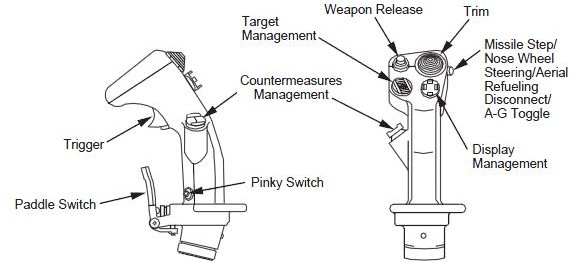
\includegraphics[width=0.65\textwidth]{F-16_Side_Stick_Controller-1.jpg}
	\caption{F-16 Throttle and Flight Stick. Image by Falconpedia (\url{falcon4.wikidot.com}), via Wikimedia Commons (\url{https://commons.wikimedia.org/wiki/File:F-16_Side_Stick_Controller.jpg}), licensed under the Creative Commons Attribution-Share Alike 3.0 Unported (CC BY-SA 3.0) license.}
	\label{fig:f16_hotas_dms_location}
\end{figure}

\paragraph*{DMS Across F-16 Blocks and Variants:}

The functionality of the DMS --- SOI selection, MFD format cycling and all associated behaviors --- is identical across all F-16 blocks and variants available in Falcon BMS. Differences in aircraft avionics do not alter DMS switch usage. For this reason, all DMS procedures in this chapter apply universally to the entire F-16 family.

\paragraph*{DMS Switch Response Characteristics:}

The DMS switch responds to short presses for all standard SOI designation and MFD format cycling functions. Sustained or long-duration holds have no effect on SOI selection or format page cycling. The sole exception is the HMCS symbology blanking toggle, which requires a DMS Down hold of approximately 0.5 second and does not affect standard SOI designation or format cycling operations (see \secref{sec:C3-S3-S3} for details).

%--------------------------------------------------------------------------
% CHAPTER 3: SECTION 3.1.1
%--------------------------------------------------------------------------
\subsection{SOI Definition and Master Mode Availability}
\label{sec:C3-S1-S1}

As introduced in \secref{sec:C2-S1}, the Sensor of Interest (SOI) is the display that currently receives HOTAS cursor slew commands and TMS actions. At any moment, only one display can be the SOI. The SOI is indicated visually by an asterisk on the HUD or a border outline on the MFD (see \secref{sec:C2-S1-S2} for complete details).

The availability of displays as valid SOI varies by master mode. \tabref{tab:C3-S1-SOI-by-mode} below shows which displays can serve as SOI in the primary operational contexts. Note that in air-to-air employment modes (A-A, DGFT, MSL OVRD), the HUD is \textbf{never} available as SOI; A-A modes \textit{restrict} the pilot to left and right MFD as the SOI. This constraint ensures that radar and tactical displays remain the primary source of truth in air-to-air engagements.

\small
\renewcommand{\arraystretch}{1.2}

\begin{longtable}{L{2.5cm} L{6.5cm} L{6.0cm}}
	\caption{SOI Availabity by Master Mode\label{tab:C3-S1-SOI-by-mode}}\\
	
	\rowcolor{headerblue}
	\textbf{\color{white}Master Mode} & \textbf{\color{white}Valid SOI Displays} & \textbf{\color{white}Constraints \& Notes} \\
	\endfirsthead
	
	\rowcolor{headerblue}
	\textbf{\color{white}Master Mode} & \textbf{\color{white}Valid SOI Displays} & \textbf{\color{white}Constraints \& Notes} \\
	\endhead
	
	\multicolumn{3}{r}{\emph{Continues on next page}}\\
	\endfoot
	
	\endlastfoot
	
	NAV (Navigation) & HUD and MFD (FCR, TGP, HSD, WPN, HAD formats) & All displays available. HUD is primary choice for situational awareness and NAV-specific tasks. \\
	A-A (Air-to-Air) & MFD only (FCR, HSD, TGP formats) & \textbf{HUD cannot be SOI.} SOI limited to radar and tactical displays. \\	
	A-G (PRE) & HUD and MFD (FCR, TGP, WPN, HAD, HSD formats) & All displays available. \\	
	A-G (VIS) & HUD and MFD (FCR, TGP, WPN formats) & Restricted to visual-capable displays. HUD used for target acquisition (e.g., AGM-65 VIS EO, DTOS, CCIP). \\	
	DGFT (Dogfight) & MFD (FCR, HSD, TGP formats) & \textbf{HUD cannot be SOI}. \\	
	MSL OVRD (Missile Override) & MFD (FCR, HSD, TGP formats) & \textbf{HUD cannot be SOI}. \\
\end{longtable}

As shown in \tabref{tab:C3-S1-SOI-by-mode}, the availability of SOI displays is strategically constrained by master mode to align pilot attention with the operational context. Navigation and air-to-ground modes offer maximum display flexibility, allowing the pilot to transition between HUD and MFD as needed.

Conversely, air-to-air and associated override modes eliminate HUD as a selectable SOI. This design reflects the fundamental principle that air-to-air engagements must be driven by primary sensor information rather than HUD-derived or symbology-based cues. However, HMCS provides an independent off-boresight capability (see \secref{sec:C3-S1-S3} for details), independent of HUD not being a valid SOI.

For visual air-to-ground delivery (VIS modes), practical SOI control --- HUD in conjunction with MFD --- focuses on visual-capable sensors: the HUD for target designation and the MFD for optical tracking (TGP format page) and weapon-specific control (WPN format page), for instance. Although the radar and optical trackings may continue to provide ranging data in the background, HUD and sensor-video-driven symbology drive the attack in VIS delivery. See \secref{sec:C3-S2-S1} for specific weapon examples (CCIP, DTOS, AGM-65 VIS EO, IAM VIS).

%--------------------------------------------------------------------------
%CHAPTER 3: SECTION 3.1.1.1
%--------------------------------------------------------------------------
\subsubsection{Valid SOI Formats}
\label{sec:C3-S1-S1-S1}

Although the MFD are capable of being SOI in any Master Mode, some MFD formats are not valid SOI because they provide information or control but do not accept sensor-like slew or targeting inputs. The table below summarizes valid and invalid SOI MFD formats.

\begin{longtable}{C{4.5cm} C{4.5cm}}
	\caption{Valid and Invalid SOI MFD Formats \label{tab:C3-S1-MFD-format}}\\
	
	\rowcolor{headerblue}
	\textbf{\color{white}Valid} & \textbf{\color{white}Invalid}\\
	\endfirsthead
	
	\rowcolor{headerblue}
	\textbf{\color{white}Valid} & \textbf{\color{white}Invalid}\\
	\endhead
	
	\multicolumn{2}{r}{\emph{Continues on next page}}\\
	\endfoot
	
	\endlastfoot
	
	Fire Control Radar (FCR); Targeting Pod (TGP); Horizontal Situation Display (HSD); HARM (HAD); Weapon (WPN) & Stores Management (SMS); Data Transfer Equipment (DTE); TEST; Blank/Inactive formats; Digital Flight Control System (FLCS); TACAN (TCN); Forward Looking Infrared (FLIR); Terrain Following Radar (TFR)
\end{longtable}

%--------------------------------------------------------------------------
% CHAPTER 3: SECTION 3.1.2
%--------------------------------------------------------------------------
\subsection{Role of DMS in SOI Selection}
\label{sec:C3-S1-S2}

The DMS manages SOI selection through two orthogonal axes of control:

\begin{itemize}
	\item \textbf{Vertical (Up / Down):} Selects \textit{which display} is SOI.
	\begin{itemize}
		\item \textbf{DMS Up:} Transfers SOI to the HUD (when permitted by master mode), detailed in \secref{sec:C3-S2}.
		\item \textbf{DMS Down:} Cycles SOI between MFD, or from HUD to an MFD, detailed in \secref{sec:C3-S3}.
	\end{itemize}
	\item \textbf{Horizontal (Left / Right):} Steps through MFD formats on the left or right MFD, independently of which display is the SOI (detailed in \secref{sec:C3-S4}).
	\begin{itemize}
		\item \textbf{DMS Left:} Cycles the left MFD format (primary $\to$ secondary $\to$ tertiary).
		\item \textbf{DMS Right:} Cycles the right MFD format (primary $\to$ secondary $\to$ tertiary).
	\end{itemize}
\end{itemize}

%--------------------------------------------------------------------------
% CHAPTER 3: SECTION 3.1.3
%--------------------------------------------------------------------------
\subsection{HUD as SOI in A-A and HMCS Capabilities}
\label{sec:C3-S1-S3}

The restriction that HUD cannot be designated as SOI in A-A master mode applies exclusively to the \textbf{SOI routing architecture} — the mechanism by which HOTAS inputs (cursor slew, TMS commands) are delivered to a specific display. This architectural constraint \textbf{does not eliminate the functional capability} of the HUD or related displays to acquire, track, or cue targets in A-A operations.

The \textbf{Helmet Mounted Cueing System (HMCS)} exemplifies this distinction. Although HMCS is an extension of the HUD display system, it shares the HUD's 
architectural restriction in A-A mode: neither can be designated as SOI via DMS. However, HMCS retains \textbf{independent off-boresight targeting capability}. For example, the pilot can slave an AIM-9 seeker to the HMCS visor line-of-sight without regard to which display (FCR, HSD, or TGP) is currently the SOI, and can employ HMCS-derived target acquisition cues that function independently of SOI status.

This principle reflects the fundamental architectural design: the SOI mechanism manages \textbf{HOTAS input routing}, while \textbf{display functional capabilities operate orthogonally}. Displays designated as SOI in A-A (FCR, HSD, TGP) receive these HOTAS inputs; displays not designated as SOI (HUD, HMCS) provide cueing and targeting functions through independent mechanisms (e.g., helmet line-of-sight, derived sensor information). Both types of functionality are essential to A-A operations, despite the SOI designation limitation.

For further technical details on HMCS capabilities and behavior in A-A contexts, refer to \dashref{2.5} (Helmet Mounted Cueing System).

%--------------------------------------------------------------------------
% CHAPTER 3: SECTION 3.2
%--------------------------------------------------------------------------
\section{DMS Up: HUD Designation as SOI}
\label{sec:C3-S2}

The \textbf{DMS Up} command attempts to designate the HUD as the Sensor of Interest (SOI). When the current master mode permits the HUD to be SOI (see \tabref{tab:C3-S1-SOI-by-mode} in \secref{sec:C3-S1}): a short press of DMS Up immediately transfers SOI to the HUD.

When DMS Up successfully designates the HUD as SOI, the HUD SOI asterisk appears and any previous MFD SOI border is removed, as described in \secref{sec:C3-S1-S1}. From that moment, all SOI-dependent HOTAS inputs (such as CURSOR/ENABLE for symbology positioning and TMS for target or waypoint designation) act on HUD symbology rather than on any MFD format. This simple visual feedback --- the HUD asterisk and loss of MFD SOI borders --- allows the pilot to confirm at a glance that all SOI-dependent commands are now applied to HUD-level cueing rather than to an MFD sensor page.

\paragraph*{Important Note:}

DMS Up is a unidirectional command to transfer SOI to the HUD. If the HUD is already the current SOI, pressing DMS Up again \textbf{has no effect} --- SOI remains on the HUD. To transition SOI from the HUD back to the MFDs, the pilot must use DMS Down (see \secref{sec:C3-S3}), not repeated DMS Up presses.

%--------------------------------------------------------------------------
% CHAPTER 3: SECTION 3.2.1
%--------------------------------------------------------------------------
\subsection{DMS Up Effectiveness}
\label{sec:C3-S2-S1}

DMS Up is only effective in master modes where the HUD is a valid SOI candidate. \tabref{tab:C3-S1-SOI-by-mode} in \secref{sec:C3-S1} summarises these constraints. This subsection focuses on the modes where HUD SOI is both permitted and operationally significant, and then contrasts them with modes where DMS Up has no effect.

%--------------------------------------------------------------------------
% CHAPTER 3: SECTION 3.2.1.1
%--------------------------------------------------------------------------
\subsubsection{Master Modes Where DMS Up is Effective (HUD as SOI Permitted)}
\label{sec:C3-S2-S1-S1}

In master modes where the HUD can be SOI, DMS Up is the hands‑on command used to designate the HUD as SOI, enabling HUD‑based visual cueing in those modes.

\paragraph*{NAV (Navigation) Master Mode:}
In Navigation mode, the HUD is the primary reference for flight path, steering, and basic situational awareness. A short press of DMS Up immediately designates the HUD as SOI. With HUD as SOI, the pilot can use SOI‑dependent HOTAS inputs to interact with navigation‑related symbology on the HUD or HMCS: CURSOR/ENABLE slews the HUD/HMCS cursor or designator, and in specific functions such as HUD or HMCS MARK, TMS Up is used to stabilise the line of sight and create markpoints, while the MFD continue to provide background information.

The exact set of displays that may become SOI in NAV, and how they compare to the HUD, is documented in \tabref{tab:C3-S1-SOI-by-mode}; DMS Up simply selects the HUD within that set.

\paragraph*{A-G in VIS (Visual Air-to-Ground)---CCIP, DTOS, AGM-65 VIS, IAM-VIS:}
In air-to-ground visual delivery modes, targets are identified and designated visually by the pilot. The HUD becomes the \textbf{primary command interface} for visual cueing, and HUD as SOI is often a prerequisite for correct TMS and CURSOR behaviour. DMS Up is therefore \textbf{operationally critical}: whenever SOI has migrated to an MFD (for example, to TGP or WPN), a short press of DMS Up restores HUD as SOI and returns HOTAS inputs to the HUD.

HUD as SOI in typical A-G VIS contexts:

\begin{itemize}
	\item \textbf{CCIP visual deliveries:} The HUD displays a pipper (computed impact point or bullet track line). The pilot maneuvers the aircraft to place the pipper on the intended impact point and commands weapon release with the weapon release button. When the fire control system allows, CURSOR/ENABLE inputs referenced to HUD SOI can be used to refine the visual aimpoint or adjust reference cues without leaving the HUD-centric view.
	\item \textbf{AGM-65 Maverick VIS:} In AGM-65 VIS, the HUD shows a target designator (TD) box that slaves the Maverick seeker. With HUD as SOI (via DMS Up), CURSOR/ENABLE slews the TD box over the intended target, and TMS Up commands seeker lock. If SOI is inadvertently left on an MFD (for example, the WPN page), TMS inputs are routed to that display instead of to the HUD TD box, and visual target rejection or re-designation through the HUD will not work as intended until DMS Up restores HUD SOI.
	\item \textbf{IAM (JSOW/JDAM) visual deliveries (IAM-VIS):} In IAM-VIS, the HUD presents a TD box and associated A-G solution cues for visual designation. With HUD as SOI, the pilot refines the TD box position by aircraft manoeuvre and, when appropriate, by CURSOR/ENABLE inputs. TMS Up then designates and ground-stabilises the target. If SOI is on an MFD, these TMS commands act on the MFD sensor page instead, and the HUD cueing will not update as expected until HUD SOI is re-established with DMS Up.
\end{itemize}

DMS Up is also valid in non‑visual A‑G modes (such as CCRP or preplanned IAM deliveries), but in those cases HUD SOI is a convenience rather than a strict requirement, since targeting, cursor management, sighting‑point control, and sensor designation can be accomplished entirely with MFD‑centric SOI (FCR, TGP, HSD). The visual modes described earlier (DTOS, AGM‑65 VIS, HUD/HMCS MARK, IAM‑VIS) are where the coupling between DMS Up and TMS/CURSOR behaviour on HUD/HMCS symbology becomes operationally critical, as these modes rely on HUD/HMCS line‑of‑sight cueing and ground‑stabilization as primary designation methods.

%--------------------------------------------------------------------------
% CHAPTER 3: SECTION 3.2.1.2
%--------------------------------------------------------------------------
\subsubsection{Modes Where DMS Up is Ineffective (HUD as SOI Prohibited)}
\label{sec:C3-S2-S1-S2}

In air-to-air employment modes (A-A, DGFT, and MSL OVRD), pressing DMS Up has no effect on SOI selection, because the HUD is not a valid SOI candidate in these modes (see \secref{sec:C3-S1-S1} and \tabref{tab:C3-S1-SOI-by-mode}). SOI remains on one of the MFD formats, such as the FCR, HSD, or TGP. The architectural rationale for this restriction, and the complementary role of HMCS in providing high off-boresight cueing in air-to-air, are developed in \secref{sec:C3-S1-S3}.

%--------------------------------------------------------------------------
% CHAPTER 3: SECTION 3.2.2
%--------------------------------------------------------------------------
\subsection{DMS Up Usage Table}
\label{sec:C3-S2-S2}

The table below summarises DMS Up behaviour across representative master modes. It should be read together with \tabref{tab:C3-S1-SOI-by-mode}, which documents which displays are valid SOI candidates in each mode.

Each table entry specifies:

\begin{itemize}
	\item \textbf{Mode}: The operational context (Master Mode).
	\item \textbf{Direction}: The physical direction for pressing the DMS hat (Up, Down, Left, Right).
	\item \textbf{Action}: The press type (Short, Long, Long Hold).
	\item \textbf{Function}: What the DMS command activates or controls.
	\item \textbf{Effect / Nuance}: The resulting system behavior, including tactics and constraints.
	\item \textbf{Dash34}: Reference section in the Dash-34 manual.
	\item \textbf{Training}: Identification of recommended BMS training mission(s) for hands-on practice (see BMS Training Manual for descriptions).
\end{itemize}

\paragraph{Training Mission Selection Rationale:} The Training column in \tabref{tab:C3-S2-DMS-Up-Usage} reflects the operational effectiveness of DMS Up in each Master Mode. The A-A row has no training missions listed, not because DMS Up is omitted from training, but because DMS Up is \textbf{ineffective} in A-A master mode. Consequently, there is no hands-on training context where DMS Up produces a meaningful result in A-A. The empty Training cell reflects this architectural constraint rather than an oversight.

\begin{hotastable}{DMS Up Usage Across NAV, A-A and A-G Master Modes}\label{tab:C3-S2-DMS-Up-Usage}
	NAV & Up & Short & Designate HUD as SOI & DMS Up is fully effective in NAV master mode. Pressing DMS Up immediately designates the HUD as SOI, placing the SOI asterisk on the HUD. With HUD/HMCS as SOI, CURSOR/ENABLE slews the HUD/HMCS cursor or designator, and in functions such as HUD or HMCS MARK, TMS Up is used to stabilise the line of sight and create markpoints. MFDs remain available for background navigation and systems information. & 2.1.1.2.3, 2.1.7.5.1, 2.1.7.5.4, 2.5.6.1 & 8, 21, 22 \\
	A-A & Up & Short & Designate HUD as SOI & DMS Up is \textbf{ineffective} in A-A master mode. The avionics architecture restricts SOI to FCR, HSD, or TGP only. HUD cannot be SOI in this mode and functions purely as a passive display. & 2.1.1.2.3 & \\
	A-G & Up & Short & Designate HUD as SOI & DMS Up is fully effective in A-G master modes. Pressing DMS Up immediately designates HUD as SOI, and an asterisk appears in the upper left corner of the HUD. \textbf{In A-G visual modes (VIS)}, HUD is the operationally critical command interface for visual target designation and rejection via CURSOR and TMS inputs. If HUD loses SOI, visual cueing control is lost and must be recovered with DMS Up. & 2.1.1.2.3, 4.2.2.1, 4.2.2.1.1 & 10, 11, 13, 14, 15 \\
\end{hotastable}

%--------------------------------------------------------------------------
% CHAPTER 3: SECTION 3.2.3
%--------------------------------------------------------------------------
\subsection{DMS Up Exception States}
\label{sec:C3-S2-S3}

In certain states, DMS Up may be temporarily ineffective even in modes where HUD is normally a valid SOI:

\begin{itemize}
	\item \textbf{Snowplow (SP) PRE state (unstabilised):} When the pilot enters Snowplow mode (a specialised ground-stabilisation mode for slewing to arbitrary ground positions) and the SP position has not yet been stabilised with TMS Up, the SOI is effectively ``nowhere''. Both the A-G radar and TGP display \texttt{NOT SOI} on the MFDs, and DMS Up/Down commands are ineffective until the SP position is stabilised. Once stabilised, SOI returns to its previous state, and DMS Up becomes effective again (\dashref{4.2.1.4}).
	\item \textbf{MARK/OFLY Submode:} In the MARK/OFLY submode (a specialised target-acquisition context documented in \dashref{2.1.1.2.3}), the SOI cannot be designated at all. As a result, DMS inputs that would normally change the SOI have no effect in this state. This exception is rare in normal operations.
\end{itemize}

%--------------------------------------------------------------------------
% CHAPTER 3: SECTION 3.3
%--------------------------------------------------------------------------
\section{DMS Down: Toggle SOI Between Displays}
\label{sec:C3-S3}

DMS Down toggles the Sensor of Interest SOI among the displays available in the current master mode. As established in \secref{sec:C3-S1-S1}, the set of valid SOI displays varies by mode: in NAV and A-G modes, the HUD is available; in air-to-air employment modes (A-A, DGFT, MSL OVRD), it is not.

Consequently, DMS Down behaves in two distinct ways:

\begin{itemize}
	\item In \textbf{NAV} and \textbf{A-G} modes, DMS Down toggles SOI through all available displays: HUD $\rightarrow$ L/R MFD $\rightarrow$ L/R MFD $\rightarrow$ HUD.
	\item In \textbf{air-to-air employment modes} (A-A, DGFT, MSL OVRD), DMS Down toggles SOI only between the two MFD (L/R MFD $\leftrightarrow$ L/R MFD), since the HUD is not a valid SOI candidate
\end{itemize}

This design ensures that DMS Up and DMS Down work together to manage SOI across all available displays in each operational context. It is \textbf{important to note} that \textbf{DMS Down} transitions SOI between displays—HUD and the two MFD—without changing which format is currently displayed on any MFD. The pilot executes hands-on commands on whatever format is available at the selected display. Format transitions \textbf{within an MFD} are controlled by DMS Right and DMS Left, covered in \secref{sec:C3-S4}.

% CHAPTER 3: SECTION 3.3.1
\subsection{DMS Down Effectiveness}
\label{sec:C3-S3-S1}
DMS Down effectiveness depends on which displays can serve as SOI in the current master 
mode, as established in \secref{sec:C3-S1-S1}.

% CHAPTER 3: SECTION 3.3.1.1
\subsubsection{Master Modes Where HUD is a Valid SOI Candidate}
\label{sec:C3-S3-S1-S1}

\paragraph{NAV (Navigation) Master Mode:}
In NAV, valid SOI candidates are the HUD and both MFD. If the HUD is SOI, DMS Down transitions SOI from HUD to the Left MFD on first press. Subsequent DMS Down presses toggle SOI between the two MFD (Left MFD $\leftrightarrow$ Right MFD). Once SOI leaves the HUD, it remains on the MFD cycle until DMS Up is pressed to restore HUD as SOI.

\paragraph{A-G in PRE (Preplanned Air-to-Ground) Mode:}
In A-G PRE, DMS Down follows the same toggle sequence as NAV (HUD $\rightarrow$ Left MFD $\leftrightarrow$ Right MFD). This allows the pilot to shift hands-on control focus between the HUD and MFD sensor pages during weapon pre-planning.

\paragraph{A-G in VIS (Visual Air-to-Ground)---CCIP, DTOS, AGM-65 VIS, IAM-VIS:}
In A-G VIS modes, valid SOI candidates are the HUD and both MFD. DMS Down toggles through the same pattern as in NAV and A-G PRE. However, in A-G VIS, DMS Down becomes \textbf{operationally critical} rather than merely convenient.

A-G VIS delivery is fundamentally HUD-centric: the pilot acquires and designates the target visually using the HUD pipper (CCIP) or target designator box (AGM-65 VIS, IAM-VIS). These visual cues are controlled by CURSOR and TMS inputs, which are routed to whichever display is currently SOI. If SOI migrates to an MFD (such as TGP for sensor refinement, WPN for weapon 
status, or FCR/HSD for situational awareness), CURSOR and TMS commands are routed to that MFD instead of the HUD. Consequently, visual designation on the HUD ceases to respond.

Therefore, \textbf{DMS Down and DMS Up} work in tandem in A-G VIS: DMS Down allows the pilot to temporarily move SOI to an MFD for sensor work or information review, while DMS Up immediately restores HUD SOI to resume visual designation. This up-down alternation is fundamental to efficient A-G VIS delivery and cannot be omitted without degrading command flow or situational awareness.

% CHAPTER 3: SECTION 3.3.1.2
\subsubsection{Modes Where HUD is NOT a Valid SOI Candidate}
\label{sec:C3-S3-S1-S2}

In air-to-air employment (A-A, DGFT, and MSL OVRD) modes, the avionics architecture restricts SOI to the MFD only. The HUD cannot be designated as SOI 
in these modes (see \secref{sec:C3-S1-S1} and \secref{sec:C3-S1-S3}). Consequently, DMS Down is limited to toggling SOI between the two MFD (L/R MFD $\leftrightarrow$ L/R MFD). This 2-way toggle allows the pilot to select which MFD sensor display receives hands-on command priority.

In A-A contexts, this is \textbf{operationally essential}: the pilot uses DMS Down to shift SOI focus between one MFD and the other so the pilot can access and have direct control over whichever format is being actually displayed: FCR for track management and missile employment, HSD for tactical picture and threat assessment or between the FCR and TGP for situational awareness or supplemental tracking. Efficient air-to-air engagement depends critically on rapid SOI management via DMS Down.

% CHAPTER 3: SECTION 3.3.2
\subsection{DMS Down Usage Table}
\label{sec:C3-S3-S2}

The table below summarises DMS Down behaviour across representative master modes. It should be read together with \tabref{tab:C3-S1-SOI-by-mode}, which documents which displays are valid SOI candidates in each mode.

Each table entry specifies:

\begin{itemize}
	\item \textbf{Mode}: The operational context (Master Mode).
	\item \textbf{Direction}: The physical direction for pressing the DMS hat (Up, Down, Left, Right).
	\item \textbf{Action}: The press type (Short, Long, Long Hold).
	\item \textbf{Function}: What the DMS command activates or controls.
	\item \textbf{Effect / Nuance}: The resulting system behavior, including tactics and constraints.
	\item \textbf{Dash34}: Reference section in the Dash-34 manual.
	\item \textbf{Training}: Identification of recommended BMS training mission(s) for hands-on practice (see BMS Training Manual for descriptions).
\end{itemize}

\begin{hotastable}{DMS Down Usage Across NAV, A-A, and A-G Master Modes}\label{tab:C3-S3-DMS-Down-Usage}
	NAV & Down & Short & Toggle SOI between HUD and MFD sensor pages & 
	DMS Down transitions SOI from HUD to L-MFD (HUD $\rightarrow$ L-MFD). Repeated presses toggle between MFDs (L-MFD $\leftrightarrow$ R-MFD). To restore HUD as SOI, press DMS Up. With HUD as SOI, hands-on commands (CURSOR/ENABLE, TMS) manage HUD navigation symbology, allowing the pilot to cycle through all available displays by alternating DMS Up/Down commands. &
	2.1.1.2.3, 2.1.6.3 &
	8, 21, 22 \\
	
	A-A & Down & Short & Toggle SOI between MFD only & 
	DMS Down toggles SOI only between the two MFD. The HUD cannot be SOI in A-A and remains a passive display. This is the primary HOTAS method for selecting which MFD sensor page receives hands-on command priority for track management, situational awareness, and weapons employment. & 
	2.1.1.2.3, 2.1.6.3 & 
	18, 17B \\
	
	A-G & Down & Short & Toggle SOI between HUD and MFD sensor pages & 
	First press transfers SOI from HUD to Left MFD (HUD $\rightarrow$ L-MFD). Subsequent presses toggle SOI between the two MFD (L-MFD $\leftrightarrow$ R-MFD). Once SOI leaves the HUD, it remains on the MFD until DMS Up is pressed to restore HUD as SOI. In A-G PRE, DMS Down is a convenience tool for shifting hands-on focus between HUD and MFD sensor pages. \textbf{In A-G VIS (CCIP, DTOS, AGM-65 VIS, IAM-VIS), DMS Down is operationally critical:} the HUD is the primary visual designation interface. DMS Down allows the pilot to alternate between HUD visual cueing (TMS/CURSOR steering, pipper control, TD box positioning) and MFD sensor work (TGP search/refine, WPN status, FCR A-G ranging). Loss of HUD as SOI in A-G VIS prevents proper visual designation and must be recovered with DMS Up, not by further DMS Down presses. & 
	2.1.1.2.3, 2.1.6.3 & 
	10, 11, 13, 14 , 15 \\
\end{hotastable}

% CHAPTER 3: SECTION 3.3.3
\subsection{DMS Down Exception States}
\label{sec:C3-S3-S3}

In certain special states and submodes, DMS Down may: (i) be temporarily ineffective, as a direct reflection of DMS Up (see \secref{sec:C3-S2-S3}):

\begin{itemize}
	\item \textbf{Snowplow (SP) PRE State (not stabilised):} As described in \secref{sec:C3-S2-S3}, the SOI is effectively ``nowhere'' in the unstabilised SP state. Consequently, \textbf{DMS Down has no effect} — the toggle mechanism has no valid display to advance SOI to. Once the SP position is stabilised with TMS Up, SOI returns to its previous display and DMS Down resumes normal toggling.
	\item \textbf{MARK/OFLY Submode:} As described in \secref{sec:C3-S2-S3}, SOI cannot be designated or changed in MARK/OFLY. \textbf{DMS Down has no effect} in this state. This submode is rare in normal operations.
\end{itemize}

Additionally, DMS Down performs a specialized function independent of SOI toggling:

\begin{itemize}
	\item \textbf{HMCS Symbology Blanking Toggle (DMS Down Hold):} 
	A sustained DMS Down press held for approximately 0.5 second toggles the HMCS between displaying symbology and blanked state. A second 0.5 second DMS Down hold restores HMCS symbology display. This feature is independent of HUD or cockpit blanking states and overrides all other blanking mechanisms. It functions only in aircraft equipped with HMCS and does not affect normal SOI designation or format cycling. See \secref{sec:C3-S1-S3} for more HMCS architectural details.
\end{itemize}

%--------------------------------------------------------------------------
%CHAPTER 3: SECTION 3.4
%--------------------------------------------------------------------------
\section{DMS Left/Right: Multifunction Display Format Cycling}
\label{sec:C3-S4}

%--------------------------------------------------------------------------
% SECTION 3.4.1
%--------------------------------------------------------------------------

\subsection{Concept}
\label{sec:C3-S4-S1}

The DMS Left and DMS Right commands are fundamentally orthogonal to the DMS Up and DMS Down controls described in \secref{sec:C3-S2} and~\secref{sec:C3-S3}. Whereas DMS Up and DMS Down select \textit{which display} (HUD, Left MFD or Right MFD) becomes the Sensor of Interest (SOI), DMS Left and DMS Right cycle through different \textit{format pages} displayed on \textit{each MFD}, independently of which display is currently designated as SOI --- \textbf{even if the HUD is the actual SOI, DMS Left/Right will actuate on each MFD}.

\paragraph{Definition of Format Cycling:}

Each MFD can display up to three different format pages, pre-configured during mission planning via the Data Transfer Cartridge (DTC) or directly by the pilot, in-flight. These three format pages are designated as PRIMARY, SECONDARY, and TERTIARY (see \secref{sec:C3-S4-S2}). DMS Left and DMS Right allow the pilot to cycle through these slots, advancing to the next format page with each button press.
%--------------------------------------------------------------------------
% SECTION 3.4.1.1
%--------------------------------------------------------------------------
\subsubsection{Format Cycling and SOI Selection --- Distinctions}
\label{sec:C3-S4-S1-S1}

The critical distinction is this: DMS Up/Down operates on the \textbf{display selection axis} (designation of which display is SOI), whereas DMS Left/Right operates on the \textbf{format pages axis} (which page is shown on an MFD). A pilot can simultaneously manage both axes:

\begin{itemize}
	
	\item Press DMS Down to transfer SOI from the Left MFD to the Right MFD (changes which display receives HOTAS commands).
	
	\item Press DMS Right to cycle the Right MFD to a different format page (changes what is displayed, independent of SOI).
	
\end{itemize}

This orthogonality is operationally powerful. The pilot can organize MFD formats for increased situational awareness while simultaneously managing which display (SOI) receives HOTAS inputs. So, pressing DMS Right changes the Right MFD format even if it is not SOI; the same applies to the Left MFD by pressing DMS Left.

The two mechanisms (SOI definition and MFD format cycling) do not interfere with each other and DMS Left/Right is not restricted by the current Master Mode.

Beyond that, DMS Left and DMS Right are \textbf{completely independent} from each other. DMS Left controls the Left MFD \textit{only}; DMS Right controls the Right MFD \textit{only}: pressing DMS Right won't, for instance, go aback to the previous left MFD format.

\begin{center}
	$\mathtt{DMS\ LEFT} \longrightarrow \mathtt{LEFT\ MFD}$\\[1em]
	$\mathtt{DMS\ RIGHT} \longrightarrow \mathtt{RIGHT\ MFD}$
\end{center}

In summary, \textbf{both MFD cycle independently and DMS Left/Right pressings don't affect SOI designation}, this is accomplished by DMS Up/Down. This independence allows the pilot to organize a visual workspace suited to the mission, so they never have to ``choose'' which display to look at or which to control; both are available simultaneously via independent mechanisms.

%--------------------------------------------------------------------------
% SECTION 3.4.2
%--------------------------------------------------------------------------
\subsection{MFD Configuration}
\label{sec:C3-S4-S2}
%--------------------------------------------------------------------------
% SECTION 3.4.2.1
%--------------------------------------------------------------------------
\subsubsection{Display Format Configuration via DTC}
\label{sec:C3-S4-S2-S1}

Each Master Mode (A-A, A-G, NAV) and also DGFT and MSL OVRD has its own independent three-slot configuration, as preset in the DTC. When the pilot switches Master Modes in-flight, the avionics automatically load the format configuration for that mode and display the chosen format. Every press of DMS Left/Right will act upon the new set of three-slot formats.

The formats can also be reconfigured by the pilot in flight, by pressing again the OSB corresponding to the actual format being displayed. See \dashref{2.1.6.2} for a comprehensive explanation.

Below is a list of every possible display pages currently present in Falcon BMS that could be configured as an MFD format, either through the DTC or by the pilot in-flight. Note that not all of them can be SOI. When selecting, in any MFD, a format that can't be designated SOI, the \textit{SOI is automatically transferred to the other MFD}.

\small
\renewcommand{\arraystretch}{1.2}

\begin{longtable}{L{1.8cm} L{4.5cm} L{7.5cm} L{2.0cm}}
	\caption{Falcon BMS Possible MFD Formats\label{table:C3-S4-S2-S1}}\\
	
	\rowcolor{headerblue}
	\textbf{\color{white}Acronym} & \textbf{\color{white}Full Name} & \textbf{\color{white}Definition} & \textbf{\color{white}Can be SOI} \\	
	\endfirsthead
	
	\rowcolor{headerblue}
	\textbf{\color{white}Acronym} & \textbf{\color{white}Full Name} & \textbf{\color{white}Definition} & \textbf{\color{white}Can be SOI} \\	
	\endhead
	
	\midrule
	\multicolumn{4}{r}{\emph{Continues on next page}}\\
	\endfoot
	
	\endlastfoot
	
	FCR & Fire Control Radar & Provides air-to-air and air-to-ground radar detection, tracking, and targeting data with multiple search and track modes for weapons employment & YES \\
	
	HSD & Horizontal Situation Display & Presents tactical navigation, situational awareness, and positioning information on a moving map display for mission planning & YES \\
	
	TGP & Targeting Pod & Displays targeting pod imagery for target acquisition, tracking, identification, and laser designation of targets & YES \\
	
	WPN & Weapon Management & Shows weapons status, aircraft ordnance configuration, and munitions management for air-to-ground missions & YES \\
	
	HAD & HARM Attack Display & Provides detection and targeting information from air defense radar sources for anti-radiation warfare missions & YES \\
	
	FLIR & Forward Looking Infrared Navigation Pod & Displays thermal imaging data for navigation, target detection, and low-level flight operations in degraded visibility & NO \\
	
	TFR & Terrain Following Radar Navigation Pod & Presents terrain elevation and clearance data for automated low-level navigation and terrain avoidance & NO \\
	
	SMS & Stores Management System & Displays current weapons configuration, loadout, and stores management parameters and status information & NO \\
	
	TCN & TACAN Format & Shows TACAN navigation aid position and bearing information for tactical air navigation and station keeping & NO \\
	
	DTE & Data Transfer Equipment & Provides interface and status for external data link communications with ground stations and other aircraft & NO \\
	
	FLCS & Digital Flight Control System & Displays flight control system parameters, status, and diagnostics for aircraft control system monitoring & NO \\
	
	TEST & Test Format & Provides system test and diagnostic pages for built-in test (BIT) functions and aircraft system verification & NO \\
	
	BLANK & Blank Format & Displays an empty/blank page with no symbology or information for display configuration flexibility & NO \\
	
\end{longtable}
%--------------------------------------------------------------------------
% SECTION 3.4.2.2
%-------------------------------------------------------------------------
\subsubsection{DTC Customization in Falcon BMS:}
\label{sec:C3-S4-S2-S2}

During mission planning in Falcon BMS (2D map screen) the pilot can access the DTC configuration by pressing its corresponding button on the right side bar (see User Manual §§ 5.1 and 9.3.4.2 for extensive explanations on DTC use in-game). In the MODES tab of the DTC configuration menu (see User Manual § 5.1.4 for extensive explanations on hot to set the formats), the pilot can assign any valid format to the three available slots of all suported modes (A-A, A-G, NAV, DGFT and MSL OVRD), and define the format (not necessarily the PRIMARY one) that will be firstly displayed on both MFD when entering that specific Master Mode in-flight.

All modifications to the DTC must be saved and loaded in the 2D map screen before taking off for any mission, as stated in the User Manual §§ 5.1.1, 5.1.9 e 9.4. These customizations are then stored in the DTC and loaded either manually or automatically when the pilot enters the 3D. They persist for the duration of the flight, unless the pilot changes them in-flight through the OSB buttons.
%--------------------------------------------------------------------------
% SECTION 3.4.2.3
%-------------------------------------------------------------------------
\subsubsection{Primary, Secondary, and Tertiary format pages}
\label{sec:C3-S4-S2-S3}

The PRIMARY, SECONDARY, and TERTIARY format pages configured by the pilot are accessed by pressing the corresponding button on the bottom row of each MFD. Each format page corresponds to one of the three central buttons in the lower OSB row of each MFD:

\begin{itemize}
	\item \textbf{OSB 14:} PRIMARY slot
	\item \textbf{OSB 13:} SECONDARY slot
	\item \textbf{OSB 12:} TERTIARY slot
\end{itemize}

The diagram below illustrates the OSB layout in the F-16 MFD:

\begin{figure}[H]
	\centering
	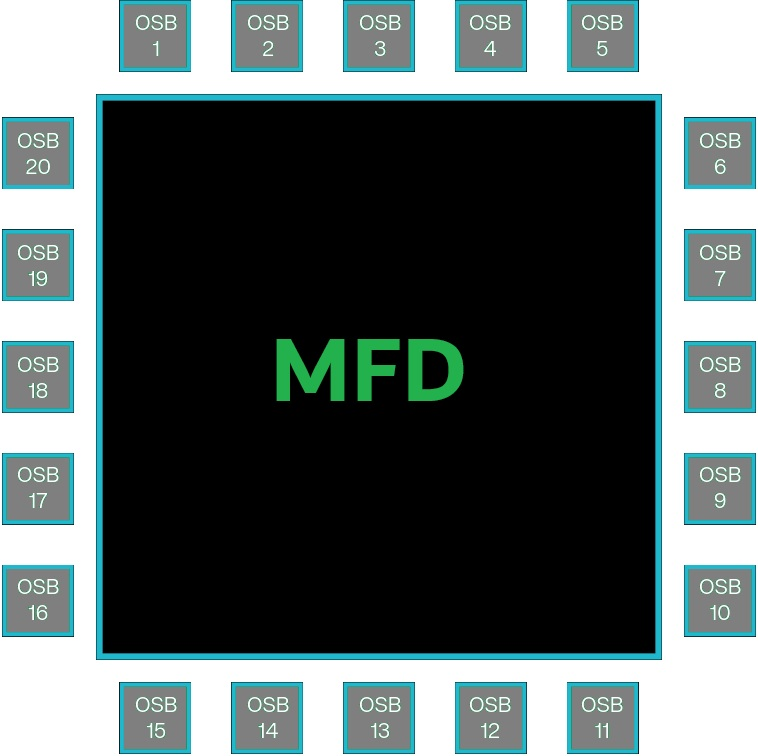
\includegraphics[width=0.36\textwidth]{MFD.jpg}
	\caption{F-16 MFD Representation. Adapted from an AI-generated image by Perplexity AI. Free to use and modify per Perplexity Terms of Service, Section 2.3.1 (\url{https://www.perplexity.ai/hub/legal/perplexity-api-terms-of-service}).}
	\label{fig:f16_MFD}
\end{figure}

Pressing the OSB corresponding to each format page is \textit{equivalent} to pressing DMS Left for the Left MDF and DMS Right for the Right MFD. When using DMS Left/Right, the formats will cycle from the inside to the outside of the MFD, in a constant sequencing, allowing pilots to develop muscle memory:

\begin{itemize}
	\item \textbf{Left MFD:} OSB 12 → OSB 13 → OSB 14
	\item \textbf{Right MFD:} OSB 14 → OSB 13 → OSB 12	
\end{itemize}

The three-slot architecture provides mission planning flexibility. During mission planning in the BMS 2D map screen, the pilot pre-configures which format pages are most useful for a given Master Mode.
%--------------------------------------------------------------------------
% SECTION 3.4.2.4
%-------------------------------------------------------------------------
\subsubsection{Cycling Constraints and Edge Cases}
\label{sec:C3-S4-S2-S4}

\paragraph{BLANK Format Skipping:}

If one or more format slots are configured as \texttt{BLANK} (meaning no format is assigned to that slot, either by choice or by default), DMS Left/Right pressings will automatically skip the BLANK format slot and advance to the next non-BLANK format slot.

\paragraph{Non-SOI-Candidate Formats:}

Some format pages are \textit{not valid} candidates for SOI designation. For example, the SMS (Stores Management System) format is not a valid SOI candidate. If a pilot customizes an MFD to include SMS in one of the three slots, and that specific MFD was SOI before cycling formats, SOI will be automatically transferred to the other MFD.

\paragraph{Format Persistence Across Master Mode Change:}

When the pilot changes Master Mode, the displayed formats on both MFD reset to the preferred formats of the actual chosen mode. There is \textit{no carryover} of the previously displayed slot.

%--------------------------------------------------------------------------
% SECTION 3.4.3: USAGE TABLE
%--------------------------------------------------------------------------

\subsection{DMS Left/Right Usage Table}
\label{sec:C3-S4-S3}

The table below summarizes DMS Left and DMS Right behavior across all Master Modes. Because format cycling is \textit{identical} in all modes, the table shows a single row for each DMS direction, applicable to every Master Mode: A-A (including DGFT and MSL OVRD), A-G and NAV.

Each table entry specifies:

\begin{itemize}
	\item \textbf{Mode}: The operational context (Master Mode).
	\item \textbf{Direction}: The physical direction for pressing the DMS hat (Up, Down, Left, Right).
	\item \textbf{Action}: The press type (Short, Long, Long Hold).
	\item \textbf{Function}: What the DMS command activates or controls.
	\item \textbf{Effect / Nuance}: The resulting system behavior, including tactics and constraints.
	\item \textbf{Dash34}: Reference section in the Dash-34 manual.
	\item \textbf{Training}: Identification of recommended BMS training mission(s) for hands-on practice (see BMS Training Manual for descriptions).
\end{itemize}

\paragraph{Training Mission Selection Rationale:} To demonstrate the operational utility of DMS Left/Right without overloading the HOTAS table, one representative mission was selected from each Master Mode (NAV, A-A, and A-G). The selection prioritized missions requiring frequent alternation between MFD formats during critical tactical phases. These three missions span the full spectrum of scenarios where DMS Left/Right provides measurable operational advantage over OSB-based navigation.

Notwithstanding the decision to present only three representative training missions, any complex mission involving A-A and A-G weapons employment will benefit from the application of DMS Left/Right.

\begin{hotastable}{DMS Left/Right Format Cycling Across All Master Modes}\label{table:dms-left-right}
	
	A-A, A-G, NAV & Left & Short & Cycle Left MFD format & DMS Left cycles the Left MFD through its configured 3-slot sequence: PRIMARY → SECONDARY → TERTIARY → PRIMARY (wrap-around). If BLANK slots are present, they are skipped automatically. Each press advances one step; no continuous cycling on hold. SOI designation of any valid display is unaffected. & 2.1.1.2.1, 2.1.6.3 & 8, 28, 18 \\
	A-A, A-G, NAV & Right & Short & Cycle Right MFD format & DMS Right cycles the Right MFD through its configured 3-slot sequence: PRIMARY → SECONDARY → TERTIARY → PRIMARY (wrap-around). If BLANK slots are present, they are skipped automatically. Each press advances one step; no continuous cycling on hold. SOI designation of any valid display is unaffected. & 2.1.1.2.1, 2.1.6.3 & 8, 28, 18 \\
	
\end{hotastable}
\newpage

%--------------------------------------------------------------------------
% CHAPTER 4: TMS (PLACEHOLDER)
%--------------------------------------------------------------------------
\chapter{TMS -- Target Management Switch}
\label{chap:C4}

\section{Concept and general behaviour}
\label{sec:C4-S1}

[Content to be developed in next phase]

\section{TMS and Situational Awareness displays}
\label{sec:C4-S2}

[Content to be developed in next phase]

\section{TMS in Air-to-Air}
\label{sec:C4-S3}

[Content to be developed in next phase]

\section{TMS in Air-to-Ground}
\label{sec:C4-S4}

[Content to be developed in next phase]

\section{TMS in weapon employment}
\label{sec:C4-S5}

[Content to be developed in next phase]

\section{TMS -- Block / variant notes}
\label{sec:C4-S6}
[Content to be developed in next phase]
\newpage

%--------------------------------------------------------------------------
% CHAPTER 5: CMS
%--------------------------------------------------------------------------
\chapter{CMS -- Countermeasures Management Switch}
\label{chap:C5}

%--------------------------------------------------------------------------
% CHAPTER 5: SECTION 5.1
%--------------------------------------------------------------------------
\section{Concept and Interaction with CMDS / ECM / RWR}\label{sec:C5-S1}

The Countermeasures Management Switch (CMS) is a four-direction hat switch mounted on the control stick that serves as the pilot's primary control interface to the F-16's integrated electronic warfare (EW) defensive systems: the ALE-47 CMDS (automatic chaff/flare dispenser), ECM systems (external pods or internal avionics), and avionics-based threat defeat systems. The CMS supervises the aircraft's defensive response by controlling defensive program selection, managing ECM operational modes, and granting or withholding consent authority to all defensive subsystems.

Its role is to grant the pilot rapid tactical control over the aircraft's defensive posture. This control is operationally critical because defensive decisions frequently occur during high-G maneuvering when hand position cannot be redirected to distant cockpit panels. A pilot executing a 6-G defensive turn cannot simultaneously reach the CMDS MODE knob on the left console or the ECM control panel without abandoning aircraft control. By placing the CMS within thumb reach during full-stick maneuver, the design ensures that no tactical scenario regardless of G-load or workload forces the pilot to choose between aircraft control and defensive system authority.

RWR, although not directly linked to CMS, is more than a display device: it is the decision engine for both CMDS and ECM. The RWR continuously evaluates detected threat radars, classifies them (SEARCH, TRACK, LAUNCH), assigns threat priority, and communicates this information to both the ALE-47 CMDS (in AUTO or SEMI mode) and the ECM system (for band selection or jamming initiation).

For in-depth explanations about CMDS, ECM and RWR operation, see \dashrefs{2.7.1, 2.7.2, and 2.7.3}, respectively. This section focuses exclusively on CMS usage and control interface. As presented in the preceding chapters, condensed diagrams of ECM and other throttle and flight stick functionalities can be found on section \dashrefs{2.1.5}. Below is an image of the F-16 Flight Stick, with the CMS switch location.

\begin{figure}[H]
\centering
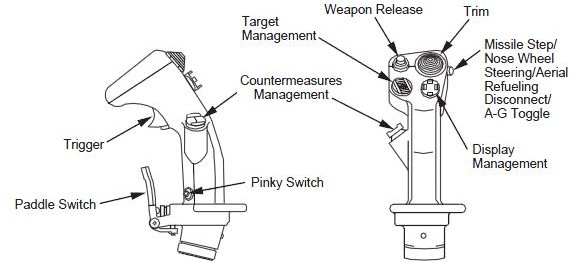
\includegraphics[width=0.65\textwidth]{F-16_Side_Stick_Controller-1.jpg}
\caption{F-16 Throttle and Flight Stick. Image by Falconpedia (\url{falcon4.wikidot.com}), via Wikimedia Commons (\url{https://commons.wikimedia.org/wiki/File:F-16_Side_Stick_Controller.jpg}), licensed under the Creative Commons Attribution-Share Alike 3.0 Unported (CC BY-SA 3.0) license.}
\label{fig:f16_hotas_cms_location}
\end{figure}

%--------------------------------------------------------------------------
% CHAPTER 5: SECTION 5.1.1
%--------------------------------------------------------------------------
\subsection{Interaction with CMDS / ECM}
\label{sec:C5-S1-S1}

Operationally, the CMS manages two distinct defensive layers: \textbf{CMDS} and \textbf{ECM} in both configurations: internal avionics and external ECM pod. The way this management is performed and all the corresponding button pressings will be detailed in the next \secref{sec:C4-S2}.

Differences in F-16 Blocks or variants, especially regarding ECM, will be discussed in \secref{sec:C5-S3}.

\begin{itemize}
  \item \textbf{ECM (External Pod):} Controls the external ECM pod's operational state through pilot-directed transmission modes and consent authority.
  \item \textbf{ECM (Integrated IDIAS):} Controls the integrated ECM system through automatic threat-reactive modes.
  \item \textbf{CMDS in Manual Mode:} Allows the pilot to execute pre-selected dispenser programs on demand, independent of automatic systems.
  \item \textbf{CMDS in Automatic/Semi-Automatic Modes:} Authorizes the ALE-47 CMDS to respond autonomously to RWR-detected threats when operating in AUTO or SEMI mode.
\end{itemize}

%--------------------------------------------------------------------------
% CHAPTER: 5 SECTION 5.2
%--------------------------------------------------------------------------
\section{CMS Switch Actuation}
\label{sec:C5-S2}

This section tabulates all CMS button combinations, organized by operational layer: Counter Measures (CMDS manual/automatic/semi modes) and Defensive Avionics integration (jamming) with both external ECM pods (ALQ-131/ALQ-184) and internal avionics (IDIAS). CMS actuation is independent of the Master Mode currently selected.

Each table entry specifies:

\begin{itemize}
  \item \textbf{Mode}: The operational context (Master Mode).
  \item \textbf{Direction}: The physical direction for pressing the CMS hat (Up, Down, Left, Right).
  \item \textbf{Action}: The press type (Short, Long, Long Hold).
  \item \textbf{Function}: What the CMS command activates or controls.
  \item \textbf{Effect / Nuance}: The resulting system behavior, including tactics and constraints.
  \item \textbf{Dash34}: Reference section in the Dash-34 manual.
  \item \textbf{Training}: Identification of recommended BMS training mission(s) for hands-on practice (see BMS Training Manual for descriptions).
\end{itemize}

% 5.2.1 CMS Actuation with CMDS
\subsection{CMS Actuation with CMDS}
\label{sec:C5-S2-S1}

The ALE-47 CMDS (Automatic Chaff and Flare Dispensing System) provides three operational modes: Manual (MAN), Automatic (AUTO), and Semi-Automatic (SEMI). Each mode grants the pilot different levels of control and autonomy over chaff and flare dispensing. The CMS is the primary interface for program execution and consent authority across all three modes.

% 5.2.1.1 Manual Mode
\subsubsection{Manual Mode}
\label{sec:C5-S2-S1-S1}

The CMDS Manual (MAN) mode grants the pilot direct, program-by-program control over countermeasure expenditure. Each CMS direction selects or executes a specific program. This mode is recommended when threat types are well-known or when chaff/flare inventory must be conserved, or by pilot choice.

\begin{hotastable}{CMS Actuation with CMDS Manual Mode}\label{tab:C5-S2-S1-S1-CMDS-Manual}
CMDS MAN & Up & Short & Execute Program 1--4 &
Runs the program selected via the CMDS panel PRGM knob once per press. No threat sensing; purely pilot-commanded. Overrides any AUTO dispensing, if running.
& 2.7.2.2 & 18, 28 \\
CMDS MAN & Left & Short & Execute Program 6 &
Flare-only program. Often pre-configured for close-range air-to-air engagements or MANPAD defense. No dependency on PRGM knob.
& 2.7.2.2 & 19 \\
\end{hotastable}

% 5.2.1.2 Automatic Mode
\subsubsection{Automatic Mode}
\label{sec:C5-S2-S1-S2}

The CMDS Automatic (AUTO) mode enables the ALE-47 CMDS to dispense chaff/flare programs continuously in response to RWR-detected threats, without requiring pilot consent for each event. Pilot consent is given once by pressing CMS Down; dispensing continues until CMS Right is pressed or expendables are exhausted.

\begin{hotastable}{CMS Actuation with CMDS Automatic Mode}\label{tab:C5-S2-S1-S2-CMDS-Auto}
CMDS AUTO & Up & Short & Execute Program 1--4 &
Manual override: runs the selected program once, interrupting any ongoing AUTO dispensing. After the manual program completes, AUTO resumes if threat persists. Useful for pilot override in high-threat scenarios.
& 2.7.2.2 & 18, 28 \\
CMDS AUTO & Left & Short & Execute Program 6 &
Manual flare-only program, overrides AUTO. After execution, AUTO resumes.
& 2.7.2.2 & 19 \\
CMDS AUTO & Down & Short & Give Consent; Enable AUTO Dispensing &
CMS Down grants consent for AUTO CMDS. RWR-detected threats trigger automatic program dispensing (selected via PRGM knob). Dispensing continues until threat clears or CMS Right is pressed. Consent state persists even if pilot switches to MAN mode; re-engaging AUTO will resume auto-dispense.
& 2.7.2.1 & 18, 28 \\
CMDS AUTO & Right & Short & Cancel Consent; Disable AUTO &
CMS Right removes CMDS consent and places the ALE-47 in Standby. Automatic dispensing halts immediately. Pilot must re-issue CMS Down to resume AUTO operation or use the system manually.
& 2.7.2.1 & 18, 28 \\
\end{hotastable}

% 5.2.1.3 Semi-Automatic Mode
\subsubsection{Semi-Automatic Mode}
\label{sec:C5-S2-S1-S3}

Semi-Automatic (SEMI) mode allows the ALE-47 to prompt the pilot for consent on a per-threat basis. When the RWR detects a threat requiring countermeasures, the CMDS displays ``DISPENSE RDY'' on the control unit and sounds a ``COUNTER'' voice message, requesting pilot consent via CMS Down.

\begin{hotastable}{CMS Actuation with CMDS Semi-Automatic Mode}\label{tab:C5-S2-S1-S3-CMDS-Semi}
CMDS SEMI & Up & Short & Execute Program 1--4 &
Manual override: runs the selected program once, independent of RWR threat state. After execution, CMDS returns to monitoring for threats and issuing ``COUNTER'' prompts.
& 2.7.2.2 & 18, 28 \\
CMDS SEMI & Left & Short & Execute Program 6 &
Manual flare-only program, independent of SEMI threat detection. After execution, CMDS resumes SEMI monitoring.
& 2.7.2.2 & 19 \\
CMDS SEMI & Down & Short & Give Consent; Dispense One Program &
When CMDS issues ``COUNTER'' (threat detected), pilot presses CMS Down to execute one instance of the selected program. If threat persists or a new threat appears, CMDS will issue ``COUNTER'' again. Consent state is tracked; switching to AUTO while consent active will trigger immediate AUTO dispensing on next threat.
& 2.7.2.1 & 18, 28 \\
CMDS SEMI & Right & Short & Cancel Consent; Return to Standby &
CMS Right removes SEMI consent. CMDS halts monitoring and returns to Standby. ``COUNTER'' messages cease.
& \dashref{2.7.2.1} & 18, 28 \\
\end{hotastable}

% 5.2.2 CMS Actuation with ECM
\subsection{CMS Actuation with ECM}
\label{sec:C5-S2-S2}

External ECM pods (ALQ-131, ALQ-184) and internal IDIAS (Improved Defensive Internal Avionic System) provide pilot-controlled jamming across frequency bands. The CMS Down position controls transmit authority for external pods; CMS Left cycles modes for internal IDIAS. Both systems interact with the RF switch and respect landing gear constraints.

% 5.2.2.1 External ECM Pod
\subsubsection{External ECM Pod (ALQ-131 / ALQ-184)}
\label{sec:C5-S2-S2-S1}

External ECM pods provide pilot-controlled jamming across five frequency-band programs. The CMS Down position grants ``ECM consent,'' enabling the pod to transmit at the XMIT switch setting (modes 1, 2, or 3). The ECM Enable light on the miscellaneous panel indicates consent state.

\begin{hotastable}{CMS Actuation with External ECM Pod}\label{tab:C5-S2-S2-S1-ECM-Pod}
ECM Pod & Down & Short & Enable ECM Transmit; Grant Consent &
CMS Down illuminates the ECM Enable light and permits the external ECM pod to transmit in the mode set by the XMIT switch on the ECM control panel (XMIT 1: AUTO Avionics Priority; XMIT 2: AUTO ECM Priority; XMIT 3: Continuous Jam). Pod continues transmitting as long as ECM is not cancelled by the pilot or RF switch is moved away from NORM.
& 2.7.4.2.5 & 28 \\
ECM Pod & Right & Short & Disable ECM Transmit; Remove Consent &
CMS Right extinguishes the ECM Enable light and places the ECM pod in Standby, halting transmission immediately. Pod will not transmit until CMS Down is re-issued.
& 2.7.4.2.5 & 28 \\
\end{hotastable}

% 5.2.2.2 Internal ECM (IDIAS)
\subsubsection{ECM (IDIAS)}
\label{sec:C5-S2-S2-S2}

Internal avionics ECM (IDIAS: Improved Defensive Internal Avionic System) automatically selects frequency bands to jam based on RWR threat priority. CMS Left cycles through operational modes (Standby, Avionics Priority, ECM Priority). CMS Down is not used for IDIAS; mode control is via CMS Left and the XMTR button on the ECM panel.

\begin{hotastable}{CMS Actuation with Internal ECM (IDIAS)}\label{tab:C5-S2-S2-S2-IDIAS}
IDIAS ECM & Left & Short & Cycle ECM Operational Mode &
Each short press of CMS Left advances the ECM mode: STBY $\rightarrow$ AVNC (Avionics Priority) $\rightarrow$ ECM (ECM Priority) $\rightarrow$ AVNC $\rightarrow$ ECM (cycles).
& 2.7.4.1.2 & 28 \\
IDIAS ECM & Right & Short & Set ECM to Standby &
CMS Right forces IDIAS ECM into STBY mode, halting all jamming operations. Requires CMS Left cycling to return to AVNC or ECM mode.
& 2.7.4.1.2 & 28 \\
\end{hotastable}

% 5.2.3 CMS Consent and Constraints
\subsection{CMS Consent and Constraints}
\label{sec:C5-S2-S3}

This subsection clarifies the relationship between CMDS consent (CMS Down) and ECM transmit authority (CMS Down for external pod). Understanding these interactions is critical for effective defensive posture management during high-workload combat operations.

\begin{hotastable}{CMS Interaction with CMDS and ECM (Consent and Constraints)}\label{tab:C5-S2-S3-CMDS-ECM}
CMDS AUTO SEMI + ECM Pod & Down & Short & Joint Consent (CMDS + ECM) &
Single CMS Down command grants consent to \textit{both} the ALE-47 CMDS (AUTO/SEMI) and the external ECM pod. There's no distinction between the two; both systems respond to the same CMS Down press. This unified control maximizes pilot situational awareness and frees workload during combat maneuvering.
& 2.7.2.1, 2.7.4.2.5 & 18, 28 \\
\end{hotastable}

% 5.2.4 Important Operational Notes
\subsection{Important Operational Notes}
\label{sec:C5-S2-S4}

The following notes clarify key behavioral interactions between CMS actuation, CMDS consent states, and ECM transmit authority. Mastery of CMS actuation across all CMDS modes (MAN, SEMI, AUTO) and ECM configurations (external pod, IDIAS) is essential for effective defensive operations. Pilots must understand the consent state model, RF switch interactions, and inventory management to avoid unintended dispensing or system saturation.

\paragraph{State Tracking:}

In AUTO and SEMI modes, the CMDS tracks the consent state even if the pilot temporarily switches to MAN mode. If the pilot gives CMS Down consent in AUTO, then switches the CMDS MODE knob to MAN, the consent state is retained. Upon re-engaging AUTO without issuing CMS Down again, the CMDS will immediately begin dispensing if a threat is detected. This behavior can be exploited for rapid mode switching during combat but may also lead to unintended dispensing if not carefully managed.

\paragraph{Bingo Quantity Behavior:}

If expendables (chaff or flare) fall to or below the bingo quantity, the CMDS will still request consent (CMS Down) and continue dispensing. The ``LOW'' and ``OUT'' voice messages alert the pilot to low or exhausted inventory, but dispensing does not automatically stop. Pilot must monitor EWS upfront pages and manually manage inventory via CMDS MAN or by pressing CMS Right to inhibit AUTO.

\paragraph{RF Switch Override:}

The RF switch on the throttle is a master control for ECM transmission. Moving the RF switch away from NORM (e.g., to QUIET or SILENT) overrides any previous CMS Down command and places both the external ECM pod and internal IDIAS in Standby. Returning RF to NORM does \textit{not} automatically restore transmission; the pilot must re-issue CMS Down.

\paragraph{Consent vs. CMDS Consent:}

The unified CMS Down consent described in \tabref{tab:C5-S2-S3-CMDS-ECM} does not apply to IDIAS-equipped aircraft: internal IDIAS uses CMS Left for mode cycling, not CMS Down. This distinction is critical for aircraft configured with IDIAS and must not be confused with the external ECM pod workflow.

\paragraph{Operations Safety:}

On the ground, ECM pods are held in Standby for safety reasons. Pilots must not hold CMS Down while on the ground in the vicinity of personnel, as the ECM pod may radiate and pose a hazard. Ground personnel must be clear before the pilot engages ECM for pre-flight high-level BIT (Built-In Test). Once airborne, ECM consent (CMS Down) can be issued and maintained as tactically required.

%--------------------------------------------------------------------------
% SECTION 5.3: CMS BLOCK / VARIANT NOTES
%--------------------------------------------------------------------------
\section{CMS Block and Variant Notes}
\label{sec:C5-S3}

\secref{sec:C5-S2} defines CMS actuation procedures for CMDS and ECM systems. 
CMS interaction with \textbf{CMDS is uniform across all F-16 blocks and variants} (see \secref{sec:C5-S2-S1}). However, \textbf{ECM configuration varies significantly by block and operator}, resulting in different CMS procedures: external ECM pods (ALQ-131/ALQ-184) use CMS Down as the transmit control, while internal IDIAS systems use CMS Left for mode cycling. These operational differences extend to panel controls (XMIT knob on external pods vs XMTR switch on IDIAS) and fundamentally change the pilot's CMS gesture sequence.

The present Section identifies which F-16 variants use which ECM configuration and maps them to the correct procedure section in \secref{sec:C5-S2-S2}. Before flight, pilots must verify their aircraft's ECM configuration to ensure they apply the correct CMS procedures and avoid dangerous habit transfer between external ECM and IDIAS variants.

% Section 5.3.1 
\subsection{ECM Configurations present in BMS}
\label{sec:C5-S3-S1}

Falcon BMS 4.38.1 implements two distinct ECM system architectures, each with different CMS actuation methods. The following paragraphs describe how the CMS interacts with each configuration and bring table depicting the blocks/variants equipped with each system architecture; detailed actuation procedures are provided in \secref{sec:C5-S2}.

% Section 5.3.1.1
\subsubsection{ECM Pods (ALQ-131 / ALQ-184)}
\label{sec:C5-S3-S1-S1}

These variants are equipped with an ECM Panel that employs manual jamming band selection. \textbf{CMS Down} provides ECM transmit consent.\\\\
The XMIT knob (3-position switch: 1, 2, 3) selects the jamming mode: XMIT 1 (Avionics Priority, AFT antenna only), XMIT 2 (ECM Priority, both FWD+AFT antennas), or XMIT 3 (Active Jam, continuous transmission independent of RWR threats). For detailed procedures, see \secref{sec:C5-S2-S2} and \dashrefs{2.7.4.1.1 and 2.7.4.2.5}.

\begin{table}[h]
\centering
\caption{External ECM Pod Blocks/Variants}
\label{tab:C5-S3-external-ecm-pods}
\small
\renewcommand{\arraystretch}{1.25}
\begin{tabular}{|>{\raggedright\arraybackslash}p{3.0cm}|>{\raggedright\arraybackslash}p{5.8cm}|}
\hline
\rowcolor{headerblue}
\textcolor{white}{\textbf{Operator}} & \textcolor{white}{\textbf{Block/Variant}} \\
\hline
USAF & Blocks 40/42/50/52 (CM designation) \\
\hline
NATO & Block 15 operators (Belgium, Denmark, Netherlands, Norway) \\
\hline
International & Egypt, Korea KF-16C Block 32 \\
\hline
\end{tabular}
\end{table}

% Section 5.3.1.2
\subsubsection{ECM (IDIAS)}
\label{sec:C5-S3-S1-S2}

These variants use the IDIAS ECM Panel. \textbf{CMS Left} to cycles all operational modes.\\\\
The XMTR switch (2-position toggle: STBY, OPER) enables the ECM system; when in OPER, the mode (AVNC, ECM or STBY) is selected via CMS Left and determines ECM behavior. For detailed procedures, see \secref{sec:C5-S2-S2} and \dashrefs{2.7.4.1.2 and 2.7.4.2.6}.
\begin{table}[h]
\centering
\caption{Internal ECM Blocks/Variants}
\label{tab:C5-S3-internal-ecm}
\small
\renewcommand{\arraystretch}{1.25}
\begin{tabular}{|>{\raggedright\arraybackslash}p{3.0cm}|>{\raggedright\arraybackslash}p{5.8cm}|}
\hline
\rowcolor{headerblue}
\textcolor{white}{\textbf{Operator}} & \textcolor{white}{\textbf{Block/Variant}} \\
\hline
Israel & F-16I Sufa Block 52, Barak I Block 30, Barak II Block 40 \\
\hline
International & Greek HAF (Blocks 50 PXII, 52 PXIII, 52+ PXIV Advanced), Korea KF-16C Block 52, Singapore F-16D Block 52 \\
\hline
\end{tabular}
\end{table}

% Section 5.3.1.3
\subsubsection{Clarification}
\label{sec:C5-S3-S1-S3}

The variants listed above represent variants available or not in Falcon BMS 4.38.1 but certailny don't reflect complete real-world inventories.
\newpage
%--------------------------------------------------------------------------
% CHAPTER 6: TRAINING REFERENCES (PLACEHOLDER)
%--------------------------------------------------------------------------
\chapter{Training references and practical flows}
\label{chap:C6}

\section{How to use this guide with BMS training missions}
\label{sec:C6-S1}

[Content to be developed in next phase]

\section{Recommended progression}
\label{sec:C6-S2}

[Content to be developed in next phase]

\section{Example flows for typical missions}
\label{sec:C6-S3}

[Content to be developed in next phase]
\newpage
%--------------------------------------------------------------------------
% CHAPTER 7: VISUAL REFERENCE (PLACEHOLDER)
%--------------------------------------------------------------------------
\chapter{HOTAS visual reference}
\label{chap:C7}

\section{F-16 HOTAS overview}
\label{sec:C7-S1}

[Content to be developed in next phase]

\section{TMS diagrams}
\label{sec:C7-S2}

[Content to be developed in next phase]

\section{DMS diagrams}
\label{sec:C7-S3}

[Content to be developed in next phase]

\section{CMS diagrams}
\label{sec:C7-S4}

[Content to be developed in next phase]

%--------------------------------------------------------------------------
% APPENDICES
%--------------------------------------------------------------------------
\appendix

\section{Block / variant overview}

\subsection{F-16CM Block 50/52}

[Content to be developed in next phase]

\subsection{F-16C/D Block 40/42}

[Content to be developed in next phase]

\subsection{F-16AM/BM MLU}

[Content to be developed in next phase]

\subsection{F-16I Sufa and Israeli variants}

[Content to be developed in next phase]

\subsection{Other export variants}

[Content to be developed in next phase]

\section{Tables index}

\subsection{TMS tables}

[To be populated]

\subsection{DMS tables}

[To be populated]

\subsection{CMS tables}

[To be populated]

\end{document}
